\documentclass[10pt,a4paper]{article}

\usepackage[T1]{fontenc}
\usepackage[utf8]{inputenc}
\usepackage{lmodern}
\usepackage{textcomp}
\usepackage[margin=2.3cm]{geometry}
\usepackage{amsmath,amssymb,amsthm}
\usepackage{graphicx}
\usepackage{booktabs}
\usepackage{array}
\usepackage{url}
\Urlmuskip=0mu plus 2mu\relax
\usepackage{xcolor}
\usepackage{microtype}
\usepackage{algorithm}
\usepackage{algpseudocode}
\usepackage[hidelinks]{hyperref}
\usepackage{orcidlink}
\usepackage{caption}
\captionsetup{font=small,labelfont=bf}
\setlength{\parskip}{0.4em}
\setlength{\parindent}{0pt}
\setlength{\emergencystretch}{2em}
\newtheorem{proposition}{Proposition}
\newtheorem{conjecture}{Conjecture}
\newtheorem{remark}{Remark}
\renewcommand{\algorithmicrequire}{\textbf{Input:}}
\renewcommand{\algorithmicensure}{\textbf{Output:}}

\graphicspath{{../figures/}}
% written by data/measure.py from b5.json: do not edit
\newcommand{\nSeeds}{8}
\newcommand{\nSeedsAbl}{5}
\newcommand{\nLambda}{20}
\newcommand{\cgIters}{15}
\newcommand{\warmIters}{30}
\newcommand{\baseIters}{30}
\newcommand{\nPix}{256}
\newcommand{\nTraps}{100}
\newcommand{\hvFront}{0.8223}
\newcommand{\hvFrontCi}{0.8198 to 0.8247}
\newcommand{\hvPub}{0.8071}
\newcommand{\hvPubCi}{0.8048 to 0.8094}
\newcommand{\hvDiff}{0.0152}
\newcommand{\hvDiffLo}{0.0125}
\newcommand{\hvDiffHi}{0.0179}
\newcommand{\hvDiffMin}{0.0110}
\newcommand{\hvDiffMax}{0.0207}
\newcommand{\hvRatio}{1.0188}
\newcommand{\hvRatioLo}{1.0154}
\newcommand{\hvRatioHi}{1.0222}
\newcommand{\hvRatioPct}{1.88}
\newcommand{\hvGeCount}{8}
\newcommand{\hvPubSeven}{0.8104}
\newcommand{\hvDiffSevenLo}{0.0097}
\newcommand{\hvDiffSevenHi}{0.0141}
\newcommand{\hvDiffSeven}{0.0119}
\newcommand{\hvGeCountSeven}{8}
\newcommand{\hvRefZeroFront}{0.8223}
\newcommand{\hvRefZeroPub}{0.8071}
\newcommand{\hvRefZeroDiff}{0.0152}
\newcommand{\hvRefZeroLo}{0.0125}
\newcommand{\hvRefZeroHi}{0.0179}
\newcommand{\hvRefZeroGe}{8}
\newcommand{\hvRefHalfFront}{0.3223}
\newcommand{\hvRefHalfPub}{0.3074}
\newcommand{\hvRefHalfDiff}{0.0149}
\newcommand{\hvRefHalfLo}{0.0122}
\newcommand{\hvRefHalfHi}{0.0176}
\newcommand{\hvRefHalfGe}{8}
\newcommand{\hvRefSevenFront}{0.1223}
\newcommand{\hvRefSevenPub}{0.1088}
\newcommand{\hvRefSevenDiff}{0.0135}
\newcommand{\hvRefSevenLo}{0.0110}
\newcommand{\hvRefSevenHi}{0.0160}
\newcommand{\hvRefSevenGe}{8}
\newcommand{\domGSMean}{4.8}
\newcommand{\domGSMin}{3}
\newcommand{\domGSMax}{7}
\newcommand{\domGSSeeds}{8}
\newcommand{\domGAAMean}{7.4}
\newcommand{\domGAAMin}{5}
\newcommand{\domGAAMax}{10}
\newcommand{\domGAASeeds}{8}
\newcommand{\domGSWMean}{0.4}
\newcommand{\domGSWMin}{0}
\newcommand{\domGSWMax}{2}
\newcommand{\domGSWSeeds}{2}
\newcommand{\domDSMean}{1.0}
\newcommand{\domDSMin}{1}
\newcommand{\domDSMax}{1}
\newcommand{\domDSSeeds}{8}
\newcommand{\domPFMean}{0.5}
\newcommand{\domPFMin}{0}
\newcommand{\domPFMax}{2}
\newcommand{\domPFSeeds}{3}
\newcommand{\domBothSeeds}{8}
\newcommand{\ptGSE}{0.816}
\newcommand{\ptGSU}{0.573}
\newcommand{\ptGAAE}{0.811}
\newcommand{\ptGAAU}{0.682}
\newcommand{\ptGSWE}{0.804}
\newcommand{\ptGSWU}{0.972}
\newcommand{\ptDSE}{0.651}
\newcommand{\ptDSU}{0.999}
\newcommand{\ptPFE}{0.793}
\newcommand{\ptPFU}{0.995}
\newcommand{\kneeE}{0.793}
\newcommand{\kneeELo}{0.791}
\newcommand{\kneeEHi}{0.795}
\newcommand{\kneeU}{1.000}
\newcommand{\kneeULo}{1.000}
\newcommand{\kneeUHi}{1.000}
\newcommand{\kneeSigma}{0.00}
\newcommand{\kneeSigmaLo}{-0.00}
\newcommand{\kneeSigmaHi}{0.00}
\newcommand{\kneeZeroSeeds}{8}
\newcommand{\eMaxFrontDelta}{0.0427}
\newcommand{\eMaxRatio}{1.054}
\newcommand{\eGainUNine}{0.0198}
\newcommand{\eGainUNinePp}{2.0}
\newcommand{\rawFactor}{126}
\newcommand{\rawShiftRel}{3.5}
\newcommand{\eMaxRatioPct}{5.4}
\newcommand{\hvRefHalfRel}{4.8}
\newcommand{\hvRefSevenRel}{12.4}
\newcommand{\seedOneGswE}{0.8086}
\newcommand{\seedOneGswU}{0.9963}
\newcommand{\seedOneNearE}{0.8093}
\newcommand{\seedOneNearU}{0.9276}
\newcommand{\eStart}{0.793}
\newcommand{\eMin}{0.793}
\newcommand{\eMaxFront}{0.8356}
\newcommand{\eMaxFrontLo}{0.8328}
\newcommand{\eMaxFrontHi}{0.8385}
\newcommand{\uMinFront}{0.015}
\newcommand{\uMinFrontLo}{0.000}
\newcommand{\uMinFrontHi}{0.030}
\newcommand{\nParetoMean}{19.9}
\newcommand{\nParetoMin}{19}
\newcommand{\nParetoMax}{20}
\newcommand{\monoESeeds}{8}
\newcommand{\monoLossSeeds}{8}
\newcommand{\monoUSeeds}{7}
\newcommand{\monoEViolMax}{0}
\newcommand{\monoLossViolMax}{0}
\newcommand{\monoUViolMax}{1}
\newcommand{\sigmaSlackMin}{1.81e-07}
\newcommand{\uSlackMin}{1.23e-06}
\newcommand{\uBoundInf}{109}
\newcommand{\uBoundPts}{160}
\newcommand{\lamSat}{0.097}
\newcommand{\lamSatLo}{0.089}
\newcommand{\lamSatHi}{0.105}
\newcommand{\identResid}{5.1e-16}
\newcommand{\identTrials}{20}
\newcommand{\identBoundSlack}{2.67e+03}
\newcommand{\rivGswHv}{0.8054}
\newcommand{\rivGswDiff}{0.0169}
\newcommand{\rivGswLo}{0.0132}
\newcommand{\rivGswHi}{0.0207}
\newcommand{\rivGswGe}{8}
\newcommand{\rivPfHv}{0.7899}
\newcommand{\rivPfDiff}{0.0324}
\newcommand{\rivPfLo}{0.0274}
\newcommand{\rivPfHi}{0.0373}
\newcommand{\rivPfGe}{8}
\newcommand{\rivGaaHv}{0.5880}
\newcommand{\rivGaaDiff}{0.2343}
\newcommand{\rivGaaLo}{0.2186}
\newcommand{\rivGaaHi}{0.2501}
\newcommand{\rivGaaGe}{8}
\newcommand{\rivUnionHv}{0.8131}
\newcommand{\rivUnionDiff}{0.0092}
\newcommand{\rivUnionLo}{0.0076}
\newcommand{\rivUnionHi}{0.0108}
\newcommand{\rivUnionGe}{8}
\newcommand{\rivUndom}{101.4}
\newcommand{\rivUndomMax}{149}
\newcommand{\frontDomMean}{5.1}
\newcommand{\frontDomMin}{4}
\newcommand{\frontDomMax}{7}
\newcommand{\hvGainPub}{0.0004}
\newcommand{\hvGainPubMax}{0.0006}
\newcommand{\diagGswThirtySeeds}{8}
\newcommand{\diagGswThirtyMean}{3.0}
\newcommand{\diagGswThirtyMin}{3}
\newcommand{\diagGswThirtyMax}{3}
\newcommand{\diagGswThirtyE}{3.58e-04}
\newcommand{\diagGswThirtyS}{1.0142}
\newcommand{\diagGswThirtyGain}{3.93e-04}
\newcommand{\diagGswHundredSeeds}{8}
\newcommand{\diagGswHundredMean}{6.4}
\newcommand{\diagGswHundredMin}{5}
\newcommand{\diagGswHundredMax}{8}
\newcommand{\diagGswHundredE}{4.90e-04}
\newcommand{\diagGswHundredS}{1.0216}
\newcommand{\diagGswHundredGain}{1.33e-03}
\newcommand{\diagPfHundredSeeds}{0}
\newcommand{\diagPfHundredMean}{0.0}
\newcommand{\diagPfHundredMin}{0}
\newcommand{\diagPfHundredMax}{0}
\newcommand{\diagPfHundredE}{1.32e-05}
\newcommand{\diagPfHundredS}{1.0000}
\newcommand{\diagPfHundredGain}{-1.32e-05}
\newcommand{\ablDefaultHv}{0.8230}
\newcommand{\ablDefaultDiff}{0.0000}
\newcommand{\ablDefaultAbs}{0.0000}
\newcommand{\ablDefaultSec}{64.2}
\newcommand{\ablDefaultUMin}{0.012}
\newcommand{\ablDefaultEMax}{0.8359}
\newcommand{\ablDefaultLamMax}{1.000}
\newcommand{\ablDefaultDom}{5.0}
\newcommand{\ablDefaultNPts}{20}
\newcommand{\ablDefaultNPar}{20.0}
\newcommand{\ablDefaultEFirst}{0.792}
\newcommand{\ablDefaultDiffLo}{0.0000}
\newcommand{\ablDefaultDiffHi}{0.0000}
\newcommand{\ablNLamFiveHv}{0.8130}
\newcommand{\ablNLamFiveDiff}{-0.0100}
\newcommand{\ablNLamFiveAbs}{0.0100}
\newcommand{\ablNLamFiveSec}{18.7}
\newcommand{\ablNLamFiveUMin}{0.015}
\newcommand{\ablNLamFiveEMax}{0.8321}
\newcommand{\ablNLamFiveLamMax}{1.000}
\newcommand{\ablNLamFiveDom}{1.6}
\newcommand{\ablNLamFiveNPts}{5}
\newcommand{\ablNLamFiveNPar}{5.0}
\newcommand{\ablNLamFiveEFirst}{0.792}
\newcommand{\ablNLamFiveDiffLo}{-0.0145}
\newcommand{\ablNLamFiveDiffHi}{-0.0054}
\newcommand{\ablNLamTenHv}{0.8188}
\newcommand{\ablNLamTenDiff}{-0.0042}
\newcommand{\ablNLamTenAbs}{0.0042}
\newcommand{\ablNLamTenSec}{34.7}
\newcommand{\ablNLamTenUMin}{0.029}
\newcommand{\ablNLamTenEMax}{0.8326}
\newcommand{\ablNLamTenLamMax}{1.000}
\newcommand{\ablNLamTenDom}{3.6}
\newcommand{\ablNLamTenNPts}{10}
\newcommand{\ablNLamTenNPar}{10.0}
\newcommand{\ablNLamTenEFirst}{0.792}
\newcommand{\ablNLamTenDiffLo}{-0.0077}
\newcommand{\ablNLamTenDiffHi}{-0.0008}
\newcommand{\ablNLamFortyHv}{0.8242}
\newcommand{\ablNLamFortyDiff}{0.0012}
\newcommand{\ablNLamFortyAbs}{0.0012}
\newcommand{\ablNLamFortySec}{134.5}
\newcommand{\ablNLamFortyUMin}{0.022}
\newcommand{\ablNLamFortyEMax}{0.8356}
\newcommand{\ablNLamFortyLamMax}{1.000}
\newcommand{\ablNLamFortyDom}{8.0}
\newcommand{\ablNLamFortyNPts}{40}
\newcommand{\ablNLamFortyNPar}{37.8}
\newcommand{\ablNLamFortyEFirst}{0.792}
\newcommand{\ablNLamFortyDiffLo}{-0.0005}
\newcommand{\ablNLamFortyDiffHi}{0.0028}
\newcommand{\ablCgFiveHv}{0.8190}
\newcommand{\ablCgFiveDiff}{-0.0040}
\newcommand{\ablCgFiveAbs}{0.0040}
\newcommand{\ablCgFiveSec}{30.3}
\newcommand{\ablCgFiveUMin}{0.058}
\newcommand{\ablCgFiveEMax}{0.8310}
\newcommand{\ablCgFiveLamMax}{1.000}
\newcommand{\ablCgFiveDom}{9.8}
\newcommand{\ablCgFiveNPts}{20}
\newcommand{\ablCgFiveNPar}{19.6}
\newcommand{\ablCgFiveEFirst}{0.792}
\newcommand{\ablCgFiveDiffLo}{-0.0084}
\newcommand{\ablCgFiveDiffHi}{0.0003}
\newcommand{\ablCgThirtyHv}{0.8235}
\newcommand{\ablCgThirtyDiff}{0.0005}
\newcommand{\ablCgThirtyAbs}{0.0005}
\newcommand{\ablCgThirtySec}{118.5}
\newcommand{\ablCgThirtyUMin}{0.013}
\newcommand{\ablCgThirtyEMax}{0.8358}
\newcommand{\ablCgThirtyLamMax}{1.000}
\newcommand{\ablCgThirtyDom}{3.6}
\newcommand{\ablCgThirtyNPts}{20}
\newcommand{\ablCgThirtyNPar}{19.8}
\newcommand{\ablCgThirtyEFirst}{0.792}
\newcommand{\ablCgThirtyDiffLo}{-0.0009}
\newcommand{\ablCgThirtyDiffHi}{0.0019}
\newcommand{\ablQuadHv}{0.8221}
\newcommand{\ablQuadDiff}{-0.0009}
\newcommand{\ablQuadAbs}{0.0009}
\newcommand{\ablQuadSec}{70.8}
\newcommand{\ablQuadUMin}{0.011}
\newcommand{\ablQuadEMax}{0.8354}
\newcommand{\ablQuadLamMax}{1.000}
\newcommand{\ablQuadDom}{6.2}
\newcommand{\ablQuadNPts}{20}
\newcommand{\ablQuadNPar}{19.6}
\newcommand{\ablQuadEFirst}{0.792}
\newcommand{\ablQuadDiffLo}{-0.0012}
\newcommand{\ablQuadDiffHi}{-0.0006}
\newcommand{\ablTargetHv}{0.8133}
\newcommand{\ablTargetDiff}{-0.0097}
\newcommand{\ablTargetAbs}{0.0097}
\newcommand{\ablTargetSec}{70.6}
\newcommand{\ablTargetUMin}{0.944}
\newcommand{\ablTargetEMax}{0.8137}
\newcommand{\ablTargetLamMax}{0.344}
\newcommand{\ablTargetDom}{8.4}
\newcommand{\ablTargetNPts}{20}
\newcommand{\ablTargetNPar}{16.4}
\newcommand{\ablTargetEFirst}{0.792}
\newcommand{\ablTargetDiffLo}{-0.0110}
\newcommand{\ablTargetDiffHi}{-0.0085}
\newcommand{\ablColdHv}{0.8134}
\newcommand{\ablColdDiff}{-0.0096}
\newcommand{\ablColdAbs}{0.0096}
\newcommand{\ablColdSec}{72.7}
\newcommand{\ablColdUMin}{0.020}
\newcommand{\ablColdEMax}{0.8281}
\newcommand{\ablColdLamMax}{1.000}
\newcommand{\ablColdDom}{13.0}
\newcommand{\ablColdNPts}{20}
\newcommand{\ablColdNPar}{20.0}
\newcommand{\ablColdEFirst}{0.792}
\newcommand{\ablColdDiffLo}{-0.0166}
\newcommand{\ablColdDiffHi}{-0.0026}
\newcommand{\ablStartGsHv}{0.8170}
\newcommand{\ablStartGsDiff}{-0.0060}
\newcommand{\ablStartGsAbs}{0.0060}
\newcommand{\ablStartGsSec}{68.2}
\newcommand{\ablStartGsUMin}{0.019}
\newcommand{\ablStartGsEMax}{0.8386}
\newcommand{\ablStartGsLamMax}{1.000}
\newcommand{\ablStartGsDom}{6.0}
\newcommand{\ablStartGsNPts}{20}
\newcommand{\ablStartGsNPar}{20.0}
\newcommand{\ablStartGsEFirst}{0.800}
\newcommand{\ablStartGsDiffLo}{-0.0084}
\newcommand{\ablStartGsDiffHi}{-0.0037}
\newcommand{\ablStartRandHv}{0.8143}
\newcommand{\ablStartRandDiff}{-0.0087}
\newcommand{\ablStartRandAbs}{0.0087}
\newcommand{\ablStartRandSec}{59.8}
\newcommand{\ablStartRandUMin}{0.012}
\newcommand{\ablStartRandEMax}{0.8334}
\newcommand{\ablStartRandLamMax}{1.000}
\newcommand{\ablStartRandDom}{9.8}
\newcommand{\ablStartRandNPts}{20}
\newcommand{\ablStartRandNPar}{18.4}
\newcommand{\ablStartRandEFirst}{0.735}
\newcommand{\ablStartRandDiffLo}{-0.0138}
\newcommand{\ablStartRandDiffHi}{-0.0036}
\newcommand{\ablRawHv}{0.8033}
\newcommand{\ablRawDiff}{-0.0197}
\newcommand{\ablRawAbs}{0.0197}
\newcommand{\ablRawSec}{62.8}
\newcommand{\ablRawUMin}{0.002}
\newcommand{\ablRawEMax}{0.8372}
\newcommand{\ablRawLamMax}{1.000}
\newcommand{\ablRawDom}{0.6}
\newcommand{\ablRawNPts}{20}
\newcommand{\ablRawNPar}{9.0}
\newcommand{\ablRawEFirst}{0.792}
\newcommand{\ablRawDiffLo}{-0.0278}
\newcommand{\ablRawDiffHi}{-0.0116}
\newcommand{\ablStartGswHHv}{0.8236}
\newcommand{\ablStartGswHDiff}{0.0006}
\newcommand{\ablStartGswHAbs}{0.0006}
\newcommand{\ablStartGswHSec}{48.0}
\newcommand{\ablStartGswHUMin}{0.017}
\newcommand{\ablStartGswHEMax}{0.8356}
\newcommand{\ablStartGswHLamMax}{1.000}
\newcommand{\ablStartGswHDom}{0.0}
\newcommand{\ablStartGswHNPts}{20}
\newcommand{\ablStartGswHNPar}{19.8}
\newcommand{\ablStartGswHEFirst}{0.810}
\newcommand{\ablStartGswHDiffLo}{-0.0008}
\newcommand{\ablStartGswHDiffHi}{0.0020}
\newcommand{\ablRawFirstU}{0.350}
\newcommand{\ablRawLaterU}{0.234}
\newcommand{\ablRawLamOne}{0.053}
\newcommand{\timeSlope}{200.5}
\newcommand{\timeIntercept}{5.4}
\newcommand{\timeRTwo}{0.943}
\newcommand{\timeN}{60}
\newcommand{\timeAlone}{53.9}
\newcommand{\timeAloneMax}{59.6}
\newcommand{\timeAloneMin}{50.8}
\newcommand{\timeAloneN}{3}
\newcommand{\timeAloneUnder}{3}
\newcommand{\timeAloneHvMatch}{0.0e+00}
\newcommand{\timePool}{56.8}
\newcommand{\dsSec}{18}
\newcommand{\consistMax}{0.0e+00}
\newcommand{\benchNThirty}{6}
\newcommand{\benchPassThirty}{5}
\newcommand{\benchWorstThirty}{-0.001}
\newcommand{\benchBestThirty}{0.014}
\newcommand{\benchWorstAbsThirty}{0.001}
\newcommand{\benchNHundred}{6}
\newcommand{\benchPassHundred}{3}
\newcommand{\benchWorstHundred}{-0.013}
\newcommand{\benchBestHundred}{0.007}
\newcommand{\benchWorstAbsHundred}{0.013}
\newcommand{\benchRows}{1326}
\newcommand{\benchSeeds}{20}
\newcommand{\benchEngine}{0.02.003}
\newcommand{\bakeSeeds}{3}


% Page-1 header block (conventions/manuscript-header-standard.md). The four document macros are set by the
% publishing tool when the version DOI is reserved.
\newcommand{\doctype}{Preprint}
\newcommand{\docversion}{v0.01}
\newcommand{\docdate}{3 November 2026}
\newcommand{\versiondoi}{10.5281/zenodo.pending}
\newcommand{\conceptdoi}{10.5281/zenodo.pending}
\newcommand{\docrepo}{github.com/fsantibanezleal/CEFOP\_DinHot}
\newcommand{\headerblock}{%
\begin{center}
\fbox{\parbox{0.94\textwidth}{\small\raggedright
\textbf{\doctype} \quad$\cdot$\quad \docversion, \docdate \quad$\cdot$\quad Licence CC BY 4.0\\[2pt]
CAOS open-research programme \quad$\cdot$\quad CEFOP\_DinHot, holographic optical trap studio\\[2pt]
Version DOI \href{https://doi.org/\versiondoi}{\texttt{\versiondoi}} \quad$\cdot$\quad
concept DOI (always latest) \href{https://doi.org/\conceptdoi}{\texttt{\conceptdoi}}\\[2pt]
Not peer reviewed. Source code, data and computational records: \href{https://\docrepo}{\texttt{\docrepo}}
}}
\end{center}
\vspace{4pt}}

\begin{document}

\title{Tracing the Efficiency-Uniformity Pareto Front of Holographic Optical Trap Arrays\\ by Continuation of a Weighted Cost}
\author{Felipe Santib\'a\~nez-Leal~\orcidlink{0000-0002-0150-3246}\\
\small CAOS open-research programme, Santiago, Chile\\
\small \texttt{fsantibanez@gmail.com}}
\date{}
\maketitle
\vspace{-1.2em}
\headerblock

\begin{abstract}
Every method that computes the hologram of an array of optical traps trades the light in the traps against their uniformity, and the literature reports one or two points of that trade-off per method and per task. We propose to compute the whole front by
continuation: a weight $\lambda$ combines a normalized squared error of the trap intensities and the normalized light into one loss, the loss is minimized by conjugate gradients at increasing weights, and each solution starts the next. An identity shows that the loss at every weight is the
squared error against a flat target raised uniformly, which gives the weight a reading and predicts the weight \lamSat{} (interval \lamSatLo{} to \lamSatHi) beyond which the target exceeds the efficiency that is reached. On a ten by ten lattice of 100 traps and \nSeeds{} seeds the front has a hypervolume of \hvFront{} against
\hvPub{} for the union of the points of Gerchberg--Saxton, the adaptive additive iteration, weighted GS and direct search run on the same seeds, a paired difference of \hvDiff{} (95 percent interval \hvDiffLo{} to \hvDiffHi) that is positive in \hvGeCount{} of \nSeeds{} seeds,
and it dominates the first two points in every seed. It dominates the weighted GS point in \domGSWSeeds{} and the phase-fixed point in \domPFSeeds{} of \nSeeds{} seeds, and \frontDomMin{} to \frontDomMax{} of its \nLambda{} points are dominated by iterates of weighted GS run for 100 iterations. In the benchmark of the studio the stored fronts meet the published union on \benchPassThirty{} of \benchNThirty{} geometries at 30 iterations and on \benchPassHundred{} of \benchNHundred{} at 100.
An ablation of twelve variants shows that the warm start, the scaling of the loss and the start from phase-fixed WGS each raise the hypervolume by \ablStartGsAbs{} to \ablRawAbs{}. The front is computed on the ideal device.
\end{abstract}

\noindent\textbf{Keywords:} holographic optical tweezers, Pareto front, continuation, conjugate gradient, weighted Gerchberg--Saxton, hypervolume.

\section{Introduction}\label{sec:intro}

A phase-only spatial light modulator (SLM) placed in the pupil plane of a lens forms an array of optical traps whose number now reaches the thousands. The largest
published array holds about 6100 atoms in about 12,000 tweezers, and the same report states that the light field is one of the limits of
the machine: the trap depth varies by 11.4 percent (standard deviation) across the sites after weighted Gerchberg--Saxton optimization, while a small calibrated array reaches a relative
standard deviation of the intensity of 0.3 percent~\cite{manetsch,chew}. The spread therefore grows with the size of the array, and the light that reaches the traps is a budget that the
experiment spends on the uniformity of the sites. Programmable neutral-atom simulators of hundreds of atoms~\cite{ebadi} and the sorting of atoms into defect-free arrays make the quality of the hologram a question of the yield of the
experiment, not of its elegance.

The hologram is computed, not designed, and every method that computes it trades two quantities against each other. The efficiency $e$ is the fraction of the input power that lands in the traps. The uniformity $u$ measures how equal the traps are.
The foundational comparison of Di Leonardo et al.\ runs the random superposition, the Gerchberg--Saxton (GS) iteration, its adaptive additive variant, direct search and the weighted GS iteration on one ten by ten lattice and lists one
point of the plane $(e,u)$ for each: GS reaches an efficiency of 0.94 and a uniformity of 0.60 in 30 iterations, the adaptive additive variant 0.93 and 0.79, direct search 0.68 and 1.00 after $7.5\times10^{5}$ trial phases, and the weighted GS iteration 0.93 and 0.99~\cite{dileonardo}.
Direct search owes its position to a scalar weight $f$ that multiplies the spread in its cost, and the source reports it at two values of that weight~\cite{dileonardo,polin}. The phase-fixed form of weighted GS, which freezes the
phases of the traps after a few iterations, reaches a modulation efficiency of 91.2 percent and a non-uniformity below 0.5 percent on 1500 foci in simulation~\cite{kim2019}.

The gap that this paper addresses is the following. Each source reports one point, or at most two, of a trade-off curve, and it reports it for its own task, so a reader cannot say what an extra percent of uniformity costs in light on a given array, nor whether
a published point lies on the best attainable curve or inside it. The weights that appear in the cost of direct search and in the amplitude-freedom method of Pasienski and DeMarco~\cite{pasienski} are scalars fixed in advance. The
literature of multiobjective optimization has methods that compute a whole Pareto front of a smooth problem by solving a family of weighted problems, each started from the solution of its neighbour, and the measures that compare fronts, such as the hypervolume~\cite{zitzler2003,beume}.
No source of the holography literature read for this paper applies them to the trap-array hologram and reports a front for a given array against the points of the published methods run on the same array.

The proposed method computes that front. A weight $\lambda\in[0,1]$ combines two dimensionless terms into one loss: the squared deviation of the trap intensities from a flat target, and the negative of the light in the traps, both scaled to be of order one.
The problem is solved at $\lambda=0$, where the hologram is the refined output of phase-fixed weighted GS, and then at a sequence of increasing values of $\lambda$, each solved by conjugate-gradient iterations that start from the solution of the previous value. The gradient of the loss is closed form through the adjoint of the point-trap projection of the engine, so no automatic differentiation is needed. The set of points
$(e,u)$ of the solutions is the front, and its hypervolume summarizes it in one number that can be compared with the area covered by the published points.

The result on the ten by ten task of the engine is the following. Over \nSeeds{} seeds the front has a hypervolume of \hvFront{} (95 percent interval \hvFrontCi) against \hvPub{} (\hvPubCi) for the union of the points of the four published methods of the acceptance criterion, a difference of
\hvDiff{} (interval \hvDiffLo{} to \hvDiffHi) that is positive in \hvGeCount{} of \nSeeds{} seeds. The front dominates the points of Gerchberg--Saxton and of the adaptive additive iteration in every seed, but it dominates the point of weighted GS in only \domGSWSeeds{} and the point of phase-fixed WGS in only \domPFSeeds{} of \nSeeds{} seeds, and \frontDomMin{} to \frontDomMax{} of its \nLambda{} points are dominated by iterates of weighted GS run for 100 iterations. Against the benchmark of the studio, the stored front meets the published union on \benchPassThirty{} of \benchNThirty{} geometries at 30 iterations and on \benchPassHundred{} of \benchNHundred{} at 100 iterations, so the result is limited to the task on which it was measured. The contributions are the following.
\begin{enumerate}
\item A front-tracing method for point-trap holograms: a normalized weighted loss, its closed-form gradient, and a continuation over the weight with a warm start from the neighbouring value (Section~\ref{sec:method}).
\item An identity that rewrites the loss at every weight as the squared error against a uniformly raised target, which gives the weight a physical reading, turns the largest efficiency that is reached into the weight beyond which the target exceeds it (a restatement of a measurement, not a prediction), and suggests a schedule of weights (Proposition~\ref{prop:shift}).
\item Three further properties that are proved: the monotonicity of the light and of the error along the weights for global minimizers (Proposition~\ref{prop:mono}), two bounds that tie the measured spread and uniformity to the value of the loss (Proposition~\ref{prop:bound}), and the size of the starting gradient of a warm start (Proposition~\ref{prop:warm}).
\item A controlled comparison with the published methods run by the same engine on the same task and seeds, including the one-parameter fronts that those methods generate when their own parameter or their iteration count is varied (Sections~\ref{sec:design} and~\ref{sec:results}).
\item An ablation of twelve variants of the front, measured by a committed script, with the continuation, the schedule, the number of points, the steps per point, the start and the scaling of the loss each varied alone (Section~\ref{sec:ablation}).
\item The scope of the result, stated with the cases where it fails: the weighted GS and phase-fixed WGS points are dominated in a minority of seeds, the stored fronts of the benchmark meet the published union only part of the time, and the front is computed for the ideal device (Sections~\ref{sec:discussion} and~\ref{sec:limits}).
\end{enumerate}
Section~\ref{sec:related} places the method among the published ones, Section~\ref{sec:problem} fixes the model, the metrics and the multiobjective problem, Section~\ref{sec:method} defines the method, Section~\ref{sec:theory} gives the propositions that explain it, and
Sections~\ref{sec:design} to~\ref{sec:ablation} give the experiments. Section~\ref{sec:repro} lists the commands that rebuild every number and figure.

\section{Related work}\label{sec:related}

\subsection{Iterative and search solvers for point traps}

The point-trap model of Di Leonardo et al.\ computes the field at each trap as a sum over SLM pixels and compares the solvers on a ten by ten lattice on a 768 by 768 pixel SLM. In simulation,
the random superposition reaches an efficiency of 0.69 and a uniformity of 0.01, plain GS 0.94 and 0.60, the adaptive additive variant with its exponent at 0.5 reaches 0.93 and 0.79, and the weighted form reaches 0.93 and 0.99 in about 30 steps,
with efficiency and uniformity above 0.9 already after 10 steps~\cite{dileonardo}. Direct search changes one pixel at a time against a cost that combines the mean intensity and the spread with a scalar weight: Polin et al.\ reached less than 5 percent deviation
on 119 quasi-periodic traps where GS and the adaptive additive variant stayed above 50 percent~\cite{polin}, and Di Leonardo et al.\ report it at two values of the weight, with 0.68 and 1.00 for the value 0.5, at a cost of $7.5\times10^{5}$ trial phases~\cite{dileonardo}.
The weight of direct search is the one place where the older literature trades the two quantities explicitly, and it does so at fixed values, one run per value.

For large arrays, Kim et al.\ observed that the weights of the weighted iteration lose their effect once the SLM-plane amplitude is replaced by the laser amplitude, and froze the focal-plane phases after an initial number of iterations; on 1500 foci they
report a modulation efficiency of 91.2 percent and a non-uniformity below 0.5 percent in simulation~\cite{kim2019}. The same family of algorithms computes the holograms of arrays of hundreds of atoms~\cite{ebadi} and of the array of about 12,000 sites that holds 6100 atoms~\cite{manetsch}.
A zero-padded GS with weighted feedback serves the rearrangement of atoms~\cite{kimoe2019}, and the three-dimensional extension of GS has been demonstrated experimentally~\cite{whyte}. Camera feedback closes the remaining gap between the model and the device:
Nogrette et al.\ lowered the root-mean-square non-uniformity of ten by ten traps from 19 percent to 1.4 percent in 20 iterations~\cite{nogrette}, and a calibrated small array reaches a relative standard deviation of 0.3 percent~\cite{chew}. All of these solvers
return one hologram per run. Their reported numbers are points of the plane of efficiency and uniformity, and the iteration count, the weight or the camera gain are the only knobs that move a point along a curve that no source plots for the task at hand.

\subsection{Cost-function holography and the device model}

A second family minimizes a cost over the field and not a fixed-point iteration. The mixed-region amplitude freedom method of Pasienski and DeMarco lowers the error on shaped targets by leaving the amplitude of a noise region free, at the price of the light that is sent to that region~\cite{pasienski}, and it has a mixing parameter that fixes the point where it sits between error and efficiency.
Conjugate-gradient minimization of a power of the intensity error, with the gradient in closed form and a line search, produces holograms for ultracold-atom traps~\cite{harte}, and a later variant controls phase and amplitude together~\cite{bowman}. Gradient methods with Wirtinger derivatives optimize any differentiable propagation model~\cite{chakravarthula}.
The device enters through the crosstalk model of Schroff et al., who convolve the phase with a fitted kernel and minimize a normalized intensity error with conjugate gradients~\cite{schroff}, and through a weighted GS modified for pixel crosstalk~\cite{persson}. Each of these methods has one loss and one scalar that sets its operating point.
The conjugate-gradient method of Harte et al.\ is the optimizer that the present method reuses at every weight, with the Fletcher--Reeves recursion and a strong-Wolfe line search as they are defined in the textbook treatment of nonlinear optimization~\cite{nocedal}.

\subsection{Learned generators of holograms}

Learned generators trade the quality of one hologram for speed and for a single forward pass. Neural holography calibrates a propagation model with a camera in the loop~\cite{peng}, DeepCGH produces multi-plane holograms with an unsupervised network~\cite{eybposh}, and tensor holography reaches video rate
with a network of small size~\cite{shi}. A network predicts one hologram for a given target; the front is a family of holograms for the same target indexed by a trade-off weight, so a learned generator that took the weight as an input would need a front like the one computed here as its training signal. None of the three sources reports the pair of efficiency and uniformity for an array of point traps as a curve.
The studio of which this method is a part also holds learned models, and the front is the kind of artifact that could train one: a table of holograms, each labelled with its position on the trade-off, for one array. The comparison of the present paper does not include a learned model, because the aim is the front itself.

\subsection{Pareto fronts in multiobjective optimization}

The weighted-sum scalarization is the oldest way to generate Pareto points: minimize a convex combination of the objectives and vary the weights~\cite{miettinen}. Its drawbacks for the generation of a Pareto set are documented~\cite{das1997}; one of them is that evenly spaced weights do not give evenly distributed points,
a property that the normal-boundary intersection method of Das and Dennis was proposed to provide for a general nonlinear multicriteria problem, with the computational efficiency of continuation-type algorithms~\cite{das1998}. Another is structural: a weighted sum with positive weights can never return a point that lies above the segment between two attainable points,
a statement that Remark~\ref{rem:convex} proves for the present problem. Evolutionary algorithms such as the strength Pareto
approach and the elitist non-dominated sorting genetic algorithm approximate a front with a population of candidates and use no gradient~\cite{zitzler1999,deb}. Numerical continuation methods follow a solution curve of a parametrized problem~\cite{allgower}, and a homotopy approach extends the idea to the manifold of Pareto-critical points of a smooth multiobjective problem~\cite{hillermeier}.
Steepest-descent methods for multicriteria problems and the multiple-gradient descent algorithm look, at a point, for a direction along which every objective decreases~\cite{fliege,desideri}.
Fronts are compared with quality indicators, and the hypervolume, the measure of the region of the objective space that a front dominates up to a reference point, is among those that the performance-assessment literature analyses~\cite{zitzler2003}; the cost of computing it as the number of objectives grows is the subject of~\cite{beume}, and in two dimensions
a sweep over the points sorted by one objective suffices (Algorithm~\ref{alg:hv}).
The same ideas have recently moved to machine learning, where the trade-off between tasks is posed as multiobjective optimization~\cite{sener}, solved with Pareto methods~\cite{lin}, and learned as a whole front by hypernetworks~\cite{navon}. The method of this paper takes the first of these ideas, the weighted sum with a warm start, applies it to an optics problem in which the weight has a physical reading
(Proposition~\ref{prop:shift}), and states with a proof and a measurement what the weighted sum guarantees there.

\subsection{Position of the proposed method}

Table~\ref{tab:related} lists the works that matter for the gap with what each assumes and where it falls short for the task of the paper, which is to report a front of efficiency against uniformity for an array of point traps and to compare it with the published points of the same array.
The method joins the starting point of Kim et al.\ and the loss and optimizer of the conjugate-gradient holography of Harte et al.\ to the continuation idea of multiobjective optimization. None of these pieces is new, and the paper does not claim a new optimizer. What it adds is the normalization that makes one weight
meaningful across arrays, the identity of Proposition~\ref{prop:shift} that gives the weight a physical reading and a schedule, and a measurement of what the front is worth against the points and the one-parameter fronts of the published methods run on the same task.

\begin{table}[t]
\centering\small
\caption{Published works that bound the gap, with what each assumes and where it falls short for reporting a front of efficiency against uniformity on one array of point traps. The last row is the proposed method.}
\label{tab:related}
\begin{tabular}{@{}p{4.2cm} p{4.3cm} p{5.6cm}@{}}
\toprule
Work & Assumes & Falls short for the gap\\
\midrule
Weighted GS~\cite{dileonardo} & ideal model, one run & one point $(e,u)$; no weight between the two quantities\\
Direct search~\cite{polin} & scalar weight $f$ in the cost & one value of $f$ per run, $7.5\times10^{5}$ trial phases at the value reported; no front\\
Phase-fixed WGS~\cite{kim2019} & ideal model; camera afterwards & the point sits at the uniform end; the cost in light is not shown\\
Mixed-region amplitude freedom~\cite{pasienski} & shaped field; free noise region & one mixing parameter; sparse point traps not treated\\
Conjugate gradient~\cite{harte,bowman} & one loss; closed-form gradient & one operating point; the front is not traced\\
Crosstalk in the loop~\cite{schroff,persson} & fitted device kernel & one loss; no trade-off weight\\
Learned generators~\cite{peng,eybposh,shi} & training set; one target & one hologram per target; no weight input\\
Weighted sums and continuation~\cite{miettinen,das1998,allgower} & smooth objectives & never applied to the hologram of a trap array\\
Continuation of the normalized loss (this paper) & ideal device, trap targets & scope measured in Sections~\ref{sec:results} and~\ref{sec:limits}\\
\bottomrule
\end{tabular}
\end{table}

\section{Problem formulation}\label{sec:problem}

\subsection{Forward model of the traps}

The SLM has $n_{\mathrm{pix}}\times n_{\mathrm{pix}}$ pixels of pitch $p$ and a Gaussian input beam of amplitude $A_j$ normalized so that $\sum_jA_j^2=n_{\mathrm{pix}}^2$. A hologram is a phase $\phi_j\in[0,2\pi)$ per pixel $j$ at
position $(x_j,y_j)$. For a trap $m$ at $(x_m,y_m)$ in the focal plane of a lens of focal length $f_{\mathrm L}$ at wavelength $\lambda_{\mathrm L}$, with the trap in the focal plane and no vortex, the field and the intensity are
\begin{equation}
V_m=\frac1{n_{\mathrm{pix}}^2}\sum_jA_je^{\,i(\phi_j-\Delta_j^m)},\qquad \Delta_j^m=\frac{2\pi}{\lambda_{\mathrm L} f_{\mathrm L}}(x_jx_m+y_jy_m),\qquad I_m=|V_m|^2,\label{eq:forward}
\end{equation}
following Di Leonardo et al.~\cite{dileonardo}. The traps lie on the bins of the zero-padded fast Fourier transform of the SLM field, so that the same field can also be read from a transform; the lattice of the task is spaced a whole number of bins apart and the
focal bin is $\lambda_{\mathrm L} f_{\mathrm L}/(\mathrm{pad}\,n_{\mathrm{pix}}\,p)$ with a padding factor $\mathrm{pad}$. Each trap has a design weight $w_m$ (equal for all traps in the task of the paper). The intensities that enter the uniformity are divided by the weights, $I_m/w_m$.
Equation~\ref{eq:forward} is the model on which every hologram of the paper is computed and scored. The engine evaluates it as a matrix product of the field with the factors of the separable phase, so that one evaluation costs $O(n_{\mathrm{pix}}^2M)$ operations for $M$ traps, and its adjoint costs the same.
The equation is linear in the unit phasors $e^{i\phi_j}$, which is what makes the gradient of any smooth function of the intensities available in closed form through the adjoint, as used in Section~\ref{sec:method}. The model is scalar and monochromatic, and the device that displays the hologram is ideal: the pixels are not blurred, the phase is not quantized and the fill factor is one.

\subsection{Figures of merit}

The efficiency is the light in the traps, and the uniformity compares the brightest and the dimmest trap, both after division by the design weights:
\begin{equation}
e=\sum_mI_m,\qquad u=1-\frac{\max_m(I_m/w_m)-\min_m(I_m/w_m)}{\max_m(I_m/w_m)+\min_m(I_m/w_m)}.\label{eq:eu}
\end{equation}
A uniformity of one means equal traps, and it falls to zero when the dimmest trap is dark. The same definition is used for the points of the published methods, so every number of the paper that has the label uniformity is computed by it. The relative standard deviation of the weighted intensities, in percent,
\begin{equation}
\sigma=100\,\frac{\operatorname{std}_m(I_m/w_m)}{\operatorname{mean}_m(I_m/w_m)}\label{eq:sigma}
\end{equation}
is the quantity that the experiments of the sources report as non-uniformity, and it is carried by the front as a third column; it is not used as the second objective because it depends on all the traps, whereas $u$ depends on two. The choice of $u$ as the objective follows the foundational comparison of
the solvers~\cite{dileonardo}, which reports the pair $(e,u)$, so the points of the published methods are in the same plane as the front. The two quantities are in conflict on the task: along every front of Section~\ref{sec:results} the efficiency rises while the uniformity falls, and Section~\ref{sec:theory} states the conflict through the loss.

\subsection{The bi-objective problem, dominance and the hypervolume}

The problem is the vector maximization of $\big(e(\phi),u(\phi)\big)$ over the phases $\phi\in[0,2\pi)^{n_{\mathrm{pix}}\times n_{\mathrm{pix}}}$. A hologram $\phi$ dominates a hologram $\phi'$ when $e(\phi)\ge e(\phi')$ and $u(\phi)\ge u(\phi')$ with at least one strict inequality,
and the Pareto front is the set of the vectors $(e,u)$ of the holograms that no hologram dominates. A finite set of points $P=\{(e_k,u_k)\}$ is summarized by its hypervolume with respect to a reference point $\mathbf r=(r_e,r_u)$, the area of the union of the rectangles that each point spans with the reference,
\begin{equation}
\mathrm{HV}(P;\mathbf r)=\Big|\bigcup_{k}\,[r_e,e_k]\times[r_u,u_k]\Big|.\label{eq:hv}
\end{equation}
The reference of the paper is $\mathbf r=(0,0)$, so that $\mathrm{HV}$ is bounded by one and a single point $(e,u)$ has $\mathrm{HV}=eu$. Two properties of the hypervolume are used. Adding a point never lowers it, and adding a dominated point leaves it unchanged, because its rectangle lies inside the rectangle of the dominating point; and if every
point of a set $A$ is dominated by or equal to some point of a set $B$, then $\mathrm{HV}(A)\le\mathrm{HV}(B)$. The hypervolume of a front is therefore a single number that is at least as large as that of any set of points the front dominates, which is what the acceptance criterion of the method needs. The converse does not hold: a front can have a hypervolume
larger than that of a set of points without dominating any single one of them, because the regions that the points add and the front adds are different. Section~\ref{sec:results} reports both the hypervolume and the point-by-point dominance for this reason.
The sensitivity of the hypervolume to the reference point is measured in Section~\ref{sec:results} with two further references.

\subsection{Task, assumptions and notation}

The task is the acceptance task of the engine: a ten by ten square lattice of $M=\nTraps$ equal traps on FFT bins 8 bins apart, a $\nPix\times\nPix$ pixel SLM of pitch 12.5~\textmu m padded by a factor 2, a Gaussian input beam, a wavelength of 850~nm and a lens of 250~mm. The lattice is the one used in the foundational
comparison of the solvers~\cite{dileonardo}, so the points of the published methods are comparable with the literature. The assumptions are the following. The traps lie in the focal plane and carry no vortex, so Eq.~\ref{eq:forward} holds exactly on the bins. The device is ideal. All weights $w_m$ are equal for the
statements of Section~\ref{sec:theory} that name equal weights, and the loss itself is defined for any weights. The published methods and the proposed one start from the same seeded random superposition of prisms and lenses~\cite{dileonardo}, drawn by the engine's portable generator, so a seed fixes the start of every method.
The three conditions are revisited in Section~\ref{sec:limits}. Table~\ref{tab:notation} collects the symbols of the paper.

\begin{table}[t]
\centering\small
\caption{Notation: every symbol of the paper with its meaning and unit. Dimensionless quantities are marked as such; intensities are fractions of the power that enters the SLM.}
\label{tab:notation}
\begin{tabular}{@{}l p{8.6cm} l@{}}
\toprule
Symbol & Meaning & Unit\\
\midrule
$n_{\mathrm{pix}}$, $p$ & SLM pixels per side, pixel pitch & 1, m\\
$\lambda_{\mathrm L}$, $f_{\mathrm L}$ & wavelength and focal length of the lens & m\\
$A_j$, $\phi_j$ & input amplitude and displayed phase of pixel $j$ & 1, rad\\
$V_m$, $I_m$ & field and intensity of trap $m$ & 1\\
$M$, $w_m$ & number of traps, design weight of trap $m$ & 1\\
$e$, $u$, $\sigma$ & efficiency, uniformity, relative standard deviation of the weighted intensities & 1, 1, percent\\
$\mathrm{HV}$, $\mathbf r$ & hypervolume, reference point of the hypervolume & 1\\
$e_0$ & efficiency of the start hologram & 1\\
$T_m$ & target intensity of trap $m$, $e_0w_m/\sum_kw_k$ & 1\\
$E$, $S$ & normalized squared error and normalized light, Eqs.~\ref{eq:E} and~\ref{eq:S} & 1\\
$\lambda$, $L_\lambda$ & weight of the front, loss at the weight $\lambda$ & 1\\
$\delta_\lambda$ & uniform raise of the target at the weight $\lambda$, Eq.~\ref{eq:delta} & 1\\
$\lambda^\ast$ & weight beyond which the shifted target exceeds the light that is attainable, Eq.~\ref{eq:lamstar} & 1\\
$n_\lambda$, $K$ & number of weights, conjugate-gradient iterations per weight & 1\\
$\tau$ & equal-weight target, $e_0/M$ & 1\\
$F_k$ & point $(e_k,u_k,\sigma_k)$ of the front at the weight $\lambda_k$ & 1\\
$\bar x$, $s$, $t_{n-1}$ & mean, sample standard deviation and Student quantile of the statistics over the seeds & as the variable\\
\bottomrule
\end{tabular}
\end{table}

\section{Proposed method: continuation of a weighted cost}\label{sec:method}

The method computes the front of the bi-objective problem of Section~\ref{sec:problem} for one array and one start, in the engine of the studio, as a sequence of smooth minimizations. It replaces the two objectives by two dimensionless functions of the intensities with closed-form gradients,
combines them with a weight, and follows the solution of the combination as the weight grows. The start is the output of phase-fixed weighted GS, the optimizer is the conjugate-gradient iteration of Harte et al.~\cite{harte}, and the new ingredients are the normalization, the warm start along the weights and the readout of the front
(its non-dominated points, its hypervolume and its knee). Each subsection gives the idea, the derivation, the algorithm, the parameters with their values and the way they were chosen, the complexity and the implementation.

\subsection{Idea}\label{sec:idea}

Every solver of Section~\ref{sec:related} stops at one point of the plane $(e,u)$, and the only knob that moves the point is a parameter fixed in advance: the weight of direct search, the mixing parameter of the amplitude-freedom method, the number of iterations. Consider instead a single loss
that contains both quantities and a weight $\lambda$ between them. At $\lambda=0$ the loss asks only for equal traps, and a hologram that minimizes it is a flat hologram of whatever efficiency the start already had. At $\lambda=1$ it asks only for light in the traps, and the minimizer ignores the uniformity.
In between, each value of $\lambda$ has a minimizer, and if the minimizers change smoothly with $\lambda$ they trace a curve in the plane $(e,u)$: the front. Two observations make this practical. First, the minimizer at a value $\lambda_{k+1}$ is close to the minimizer at $\lambda_k$ when the values are close, so each
minimization can start from its neighbour and needs only a few conjugate-gradient steps (a quantitative statement is Proposition~\ref{prop:warm}). Second, the two terms must be scaled so that one weight means the same on every array: the squared error of the intensities without division is $E\sum_kT_k^2$, and $\sum_kT_k^2=e_0^2/M$ is of the order of $6\times10^{-3}$ for a hundred traps, while the light is of order one,
so a loss without scaling asks for a raise of every trap that is $M/e_0$ times larger than the scaled loss asks for the same weight (Proposition~\ref{prop:shift}) and the front collapses toward the efficient end at the first weights; the ablation of Section~\ref{sec:ablation} measures this collapse. The scaling divides the error by the squared norm of the target and the light by the efficiency of the start, so both terms are of order one and
the weight $\lambda=1/2$ is a balanced choice by construction.

The weight has a physical reading that the derivation exposes. Completing the square shows that, up to a constant, the loss at weight $\lambda$ is the squared error against a flat target whose every trap is raised by a fixed amount $\delta_\lambda$ that grows with $\lambda$ (Proposition~\ref{prop:shift}).
The weight therefore sets how much more light than the start the hologram is asked to put in each trap while keeping the traps equal. The front is then the set of best approximations to a family of flat targets of increasing brightness, and it ends where the requested brightness exceeds what the optics allow, a weight that the proposition computes
from the efficiency of the start and the largest efficiency reached (it restates that measurement and is not a prediction).

\subsection{Derivation}\label{sec:derivation}

Let $V_m(\phi)$ be the trap fields of Eq.~\ref{eq:forward}, $I_m=|V_m|^2$, and $e_0$ the efficiency of the start hologram $\phi^{(0)}$ that is the output of phase-fixed weighted GS. The target intensities have the total light of the start and the proportions of the design weights,
\begin{equation}
T_m=e_0\,\frac{w_m}{\sum_kw_k},\qquad \sum_mT_m=e_0.\label{eq:target}
\end{equation}
Two functions of the hologram are defined, the normalized squared error of the intensities against the target and the light in the traps relative to the start,
\begin{equation}
E(\phi)=\frac{\sum_m\big(I_m-T_m\big)^2}{\sum_mT_m^2},\label{eq:E}
\end{equation}
\begin{equation}
S(\phi)=\frac{\sum_mI_m}{e_0}=\frac{e(\phi)}{e_0}.\label{eq:S}
\end{equation}
Both are dimensionless. $E$ vanishes when the traps equal the target, and $S$ equals one for the start. The loss at the weight $\lambda\in[0,1]$ is the convex combination of the quantity to be minimized, $E$, and the negative of the quantity to be maximized, $S$,
\begin{equation}
L_\lambda(\phi)=(1-\lambda)\,E(\phi)-\lambda\,S(\phi).\label{eq:loss}
\end{equation}
The loss is a function of the intensities only, so it is unchanged by a global phase of the field, and the normalizations make it independent of the scale of the target and of the number of traps to first order: $E$ is the mean over traps of the squared relative deviation $(I_m-T_m)^2/T_m^2$ when the weights are equal.
The form in the research record of the engine does not divide the two terms, and it is measured as a variant in Section~\ref{sec:ablation}.

The gradient is obtained in two steps. With $g_m=\partial L_\lambda/\partial I_m$,
\begin{equation}
g_m=\frac{2(1-\lambda)\,(I_m-T_m)}{\sum_kT_k^2}-\frac{\lambda}{e_0},\label{eq:gm}
\end{equation}
and since $I_m=V_m\overline{V_m}$ and $V_m$ is linear in the phasors $f_j=A_je^{i\phi_j}$ with $\partial V_m/\partial\phi_j=i f_je^{-i\Delta_j^m}/n_{\mathrm{pix}}^2$, the chain rule gives
\begin{equation}
\frac{\partial L_\lambda}{\partial\phi_j}=\sum_mg_m\frac{\partial I_m}{\partial\phi_j}=2\operatorname{Re}\Big(i\,f_j\,\overline{h_j}\Big),\qquad h_j=\frac1{n_{\mathrm{pix}}^2}\sum_mg_m\,V_m\,e^{i\Delta_j^m}.\label{eq:grad}
\end{equation}
The vector $h$ is the back-projection of the weighted fields $g_mV_m$ to the SLM plane, which is the adjoint of the projection of Eq.~\ref{eq:forward}; it costs one evaluation of the same kind as the forward field and no automatic differentiation is needed. The engine tests the gradient of the loss against
central finite differences at $\lambda=0$, $0.4$ and $1$, and the test requires a relative agreement of $10^{-5}$ in five random directions.

At each weight the loss is minimized by the Fletcher--Reeves nonlinear conjugate-gradient iteration with a strong-Wolfe line search, the optimizer that Harte et al.\ use for holographic traps~\cite{harte},
\begin{equation}
d_i=-g_i+\beta_i d_{i-1},\quad \beta_i=\frac{g_i^{\top}g_i}{g_{i-1}^{\top}g_{i-1}},\quad \phi_{i+1}=\phi_i+\alpha_i d_i,\label{eq:cg}
\end{equation}
where $g_i=\nabla_\phi L_\lambda(\phi_i)$ here denotes the gradient of Eq.~\ref{eq:grad} (the symbol $g_m$ above is the derivative with respect to the intensity of trap $m$, and the two never appear together). The step $\alpha_i$ satisfies the strong Wolfe conditions,
\begin{equation}
L_\lambda(\phi_i+\alpha_i d_i)\le L_\lambda(\phi_i)+c_1\alpha_i g_i^{\top}d_i,\qquad \big|\nabla L_\lambda(\phi_i+\alpha_i d_i)^{\top}d_i\big|\le c_2\,\big|g_i^{\top}d_i\big|,\label{eq:wolfe}
\end{equation}
with $c_1=10^{-4}$ and $c_2=0.1$; the choice $c_2<1/2$ keeps the Fletcher--Reeves direction a descent direction~\cite{nocedal}. The loss never increases along the iteration, and a restart from the steepest descent direction is taken when a direction fails to be a descent direction.

The continuation is the repeated use of this minimization along an increasing sequence of weights $0=\lambda_0<\lambda_1<\dots<\lambda_{n_\lambda-1}=1$. The hologram at $\lambda_0$ is the start refined by $K$ iterations of Eq.~\ref{eq:cg} on $L_0=E$, and the hologram at $\lambda_{k+1}$ is the result of $K$ iterations that start from the hologram at $\lambda_k$,
\begin{equation}
\phi^{(k+1)}=\mathrm{CG}_K\big(L_{\lambda_{k+1}},\,\phi^{(k)}\big),\qquad \phi^{(0)}=\mathrm{CG}_K\big(L_{\lambda_0},\,\phi_{\mathrm{start}}\big).\label{eq:continuation}
\end{equation}
The points of the front are $F_k=\big(e(\phi^{(k)}),u(\phi^{(k)})\big)$, with the relative standard deviation $\sigma_k$ of Eq.~\ref{eq:sigma} recorded as a third column. The readout of the front keeps the non-dominated points of the set $\{F_k\}$, their hypervolume (Eq.~\ref{eq:hv}), and a representative point, the knee,
\begin{equation}
k^{\star}=\arg\max_k\,e(\phi^{(k)})\,u(\phi^{(k)}),\label{eq:knee}
\end{equation}
which is the point whose rectangle against the origin has the largest area. The knee is the hologram that the engine returns as the single result of the method, and the front is returned alongside it. In the two-dimensional case the hypervolume is computed by a sweep over the points sorted by decreasing efficiency,
\begin{equation}
\mathrm{HV}=\sum_{k}\big(e_{(k)}-e_{(k+1)}\big)\,\max_{l\le k}u_{(l)},\qquad e_{(M'+1)}=r_e,\label{eq:hvsweep}
\end{equation}
where $(e_{(k)},u_{(k)})$ are the points of $F$ above the reference, sorted so that $e_{(1)}\ge e_{(2)}\ge\dots$, and the running maximum of the uniformity makes dominated points contribute nothing.

\subsection{Algorithm}\label{sec:algorithm}

Algorithm~\ref{alg:front} states the continuation and Algorithm~\ref{alg:hv} the readout. The start is $K_{\mathrm{warm}}$ iterations of phase-fixed weighted GS from the seeded random superposition, with the phases of the traps frozen at iteration $n_{\mathrm{fix}}=12$ as in the rule of Kim et al.~\cite{kim2019};
this is the engine's own implementation of that method, the same code that produces the published point of phase-fixed WGS in the comparison, so that the point of that method on a seed is exactly the start of the front on that seed. The first weight $\lambda_0=0$ asks only for equal traps at the total light of the start, and its minimizer differs from the start by the small refinement that $K$ conjugate-gradient iterations on $E$ make; every later weight raises the target.
In line~4 of Algorithm~\ref{alg:front} the weights are linear in the index, which is the default of the module, and the ablation replaces the line by two other schedules. The phases stored in line~6 are the ones returned by the engine; the front itself is the list of the points $F_k$, and the holograms are kept so that any point of the front can be displayed or refined.

\begin{algorithm}[t]
\caption{Front by continuation of the weighted cost. Inputs are the traps with their weights, the number of weights $n_\lambda$, the conjugate-gradient iterations $K$ per weight, the start iterations $K_{\mathrm{warm}}$ and a seed.}
\label{alg:front}
\begin{algorithmic}[1]
\Require traps $\{x_m,w_m\}$ on FFT bins, $n_\lambda\ge2$, $K$, $K_{\mathrm{warm}}$, seed
\Ensure front $\{F_k\}$, non-dominated indices, hypervolume, knee hologram
\State $\phi\gets K_{\mathrm{warm}}$ iterations of phase-fixed weighted GS from the random superposition of the seed
\State $e_0\gets e(\phi)$; build $T_m$ by Eq.~\ref{eq:target}
\For{$k=0,\dots,n_\lambda-1$}
  \State $\lambda_k\gets k/(n_\lambda-1)$
  \State $\phi\gets K$ iterations of Fletcher--Reeves conjugate gradients on $L_{\lambda_k}$ from $\phi$ \Comment{Eqs.~\ref{eq:loss},~\ref{eq:grad},~\ref{eq:cg}}
  \State store $\phi^{(k)}\gets\phi \bmod 2\pi$ and $F_k\gets(e,u,\sigma)$ of $\phi$ \Comment{warm start for the next weight}
\EndFor
\State $\mathcal P\gets$ non-dominated indices of $\{(e_k,u_k)\}$; $\mathrm{HV}\gets$ Algorithm~\ref{alg:hv}; $k^\star\gets\arg\max_k e_ku_k$
\State \Return $\{F_k\}$, $\mathcal P$, $\mathrm{HV}$, $\phi^{(k^\star)}$
\end{algorithmic}
\end{algorithm}

\begin{algorithm}[t]
\caption{Hypervolume of a set of points in the plane $(e,u)$ by a sweep over the points sorted by efficiency, with the reference point $\mathbf r$. Points that are not above the reference in both coordinates are discarded.}
\label{alg:hv}
\begin{algorithmic}[1]
\Require points $P=\{(e_k,u_k)\}$, reference $\mathbf r=(r_e,r_u)$
\Ensure $\mathrm{HV}(P;\mathbf r)$
\State $P'\gets\{p\in P:e>r_e,\ u>r_u\}$; sort $P'$ by decreasing $e$; $A\gets0$; $b\gets r_u$
\For{$k=1,\dots,|P'|$}
  \State $b\gets\max(b,u_{(k)})$ \Comment{best uniformity among the points at least as efficient}
  \State $e_{\mathrm{next}}\gets e_{(k+1)}$ if $k<|P'|$ else $r_e$
  \State $A\gets A+\big(e_{(k)}-\max(e_{\mathrm{next}},r_e)\big)\,(b-r_u)$
\EndFor
\State \Return $A$
\end{algorithmic}
\end{algorithm}

\subsection{Parameters}\label{sec:parameters}

Table~\ref{tab:params} lists the parameters and the origin of each value. The number of weights is the setting of the module and of the acceptance test; the number of conjugate-gradient iterations per weight is the budget of the acceptance test and the iteration count that the benchmark varies;
the start is the output of the phase-fixed rule with the freezing iteration of Kim et al.~\cite{kim2019}; the line-search constants follow the textbook choice for Fletcher--Reeves~\cite{nocedal}. The sensitivity to the number of weights, to the steps per weight, to the schedule of the weights and to the start is measured in the ablation of
Section~\ref{sec:ablation}; the constants of the line search and the reference point of the hypervolume are not varied, and the reference point is varied only in the sensitivity analysis of the hypervolume.

\begin{table}[t]
\centering\small
\caption{Parameters of the method with their values in the engine and the origin of each value; the first block holds the settings that the ablation varies, the second the constants that it does not.}
\label{tab:params}
\begin{tabular}{@{}p{4.6cm} p{3.6cm} p{5.8cm}@{}}
\toprule
Parameter & Value & Origin\\
\midrule
Weights $n_\lambda$ & \nLambda{} on $[0,1]$, linear & module default and the acceptance test\\
Steps per weight $K$ & \cgIters{} & budget of the acceptance test\\
Start iterations $K_{\mathrm{warm}}$ & \warmIters{} of phase-fixed WGS, $n_{\mathrm{fix}}=12$ & the uniform end; freezing iteration of the source of the rule~\cite{kim2019}\\
Targets and scaling & $T_m$ of Eq.~\ref{eq:target}, divisions by $\sum T^2$ and $e_0$ & definition of the method\\
\midrule
Line search & strong Wolfe, $c_1=10^{-4}$, $c_2=0.1$, at most 25 evaluations & textbook values for Fletcher--Reeves~\cite{nocedal}\\
Reference of the hypervolume & $(0,0)$ & the usual choice for two maximized objectives; varied in Section~\ref{sec:results}\\
Representative point & knee, Eq.~\ref{eq:knee} & definition of the method\\
Device & ideal; a device argument is accepted and ignored & scope of the method\\
\bottomrule
\end{tabular}
\end{table}

\subsection{Complexity}\label{sec:complexity}

One evaluation of the loss and its gradient is one forward projection and one back-projection, $O(n_{\mathrm{pix}}^2M)$ each for $M$ traps in the separable form of the engine. A conjugate-gradient iteration takes one to a few evaluations in its line search, bounded by 25, so with $c$ the mean number of evaluations per iteration the cost of the front is
\begin{equation}
T_{\mathrm{front}}\approx K_{\mathrm{warm}}\,c_{\mathrm{GS}}\,n_{\mathrm{pix}}^2M\;+\;n_\lambda K\,c\,n_{\mathrm{pix}}^2M,\label{eq:cost}
\end{equation}
where $c_{\mathrm{GS}}$ is the cost of one iteration of phase-fixed WGS in units of one evaluation. The front is $n_\lambda$ times the cost of one conjugate-gradient run of $K$ iterations, which is the cost quoted in the research record as the number of weights times a warm-started run.
The cost is linear in $n_\lambda K$; Section~\ref{sec:results} fits the measured seconds against $n_\lambda K$ over the runs of the ablation. The memory is $O(n_{\mathrm{pix}}^2+n_{\mathrm{pix}}\,c_{\mathrm{ch}})$ with $c_{\mathrm{ch}}$ the chunk of traps of the separable product, plus the $n_\lambda$ stored holograms. The sweep of Algorithm~\ref{alg:hv} costs
$O(n_\lambda\log n_\lambda)$, and the non-dominated filter of the engine, which compares every point with every other, $O(n_\lambda^2)$; both are negligible against Eq.~\ref{eq:cost}.

\subsection{Implementation}\label{sec:implementation}

The method is the module \texttt{b5\_pareto} of the beyond-methods package of the engine, with the entry \texttt{run} and the public functions \texttt{pareto\_indices} and \texttt{hypervolume}. The cost and its gradient are the class \texttt{\_FrontCost}, which uses the trap forward model and the conjugate-gradient routine of the shared optimization module of the engine, so the line search of Eq.~\ref{eq:wolfe} is the routine's own. The result carries the knee hologram, one history entry per weight with the weight, the trap fields of the knee, and in its metadata the weights, the front, the indices of the non-dominated points, the hypervolume, the knee index, all holograms and $e_0$. A target that is a shaped field is refused with an error that names the supported kind, and fewer than two weights is refused.
When a wall-clock budget is given, the iteration in progress stops at the deadline and no further weight is started, so the front is shorter; the benchmark of the studio runs its converged row with 300 iterations per weight and a limit of 20 s, and the stored fronts end at weights below one, as Section~\ref{sec:results} lists. The method has no live port: its lane is baked, and the studio's browser engine does not run it. The unit tests of the module check the hypervolume on known values,
the non-dominated indices, the gradient against finite differences, the monotone direction of the front on a small array, the refusal of a shaped field, determinism for a seed, and the acceptance criterion on the ten by ten task. The numbers of this paper do not come from the tests: they come from the script of Section~\ref{sec:repro}, which calls the module and checks that its own loop reproduces the module's front for the first seed.

\section{Theory: what the weighted loss guarantees}\label{sec:theory}

This section states what can be proved about the loss of Eq.~\ref{eq:loss} and the continuation of Eq.~\ref{eq:continuation}, and what stays a conjecture supported by measurement. The propositions concern the loss objectives $E$ and $S$ of Eqs.~\ref{eq:E} and~\ref{eq:S}; the figures of merit $e$ and $u$ of
Eq.~\ref{eq:eu} are related to them in Proposition~\ref{prop:bound}. The conditions under which each statement holds are part of it, and the last subsection lists them.

\subsection{The weight raises the target uniformly}

\begin{proposition}[shifted target]\label{prop:shift}
For $\lambda\in[0,1)$ define
\begin{equation}
\delta_\lambda=\frac{\lambda}{2(1-\lambda)}\,\frac{\sum_mT_m^2}{e_0}.\label{eq:delta}
\end{equation}
Then for every hologram $\phi$,
\begin{equation}
L_\lambda(\phi)=\frac{1-\lambda}{\sum_kT_k^2}\sum_m\big(I_m-T_m-\delta_\lambda\big)^2\;-\;\frac{1-\lambda}{\sum_kT_k^2}\Big(2\delta_\lambda\sum_mT_m+M\delta_\lambda^2\Big).\label{eq:shift}
\end{equation}
The second term does not depend on $\phi$. When the weights are equal, $T_m=\tau=e_0/M$, $\delta_\lambda=\tau\,\lambda/(2(1-\lambda))$ and the shifted target has the total light $e_0\,\big(1+\lambda/(2(1-\lambda))\big)$.
\end{proposition}
\begin{proof}
Write $a=(1-\lambda)/\sum_kT_k^2$ and $b=\lambda/e_0$, so that $L_\lambda=a\sum_m(I_m-T_m)^2-b\sum_mI_m$ and $b/a=2\delta_\lambda$ by Eq.~\ref{eq:delta}. For each trap, $(I_m-T_m)^2-2\delta_\lambda I_m=(I_m-T_m-\delta_\lambda)^2-2\delta_\lambda T_m-\delta_\lambda^2$, which is checked by expanding the square.
Summing over the traps and multiplying by $a$ gives Eq.~\ref{eq:shift}. For equal weights $\sum_kT_k^2=e_0^2/M$ and $\delta_\lambda=\lambda e_0/(2(1-\lambda)M)$, and the total of the shifted target is $e_0+M\delta_\lambda$.
\end{proof}

The proposition has three consequences that the experiments use. First, a minimizer of $L_\lambda$ is the best approximation, in the sense of the sum of squares, of a flat target that is brighter than the start by the factor $1+\lambda/(2(1-\lambda))$ in the total, so the weight $\lambda=1/2$ asks for 50 percent more light than the start and
$\lambda=2/3$ asks for twice as much. Second, because the efficiency of any hologram is bounded, there is a weight beyond which the target is out of reach. If $e_{\max}$ is the largest efficiency that the minimizers reach and $r=e_{\max}/e_0-1$, the shifted target equals that largest efficiency at
\begin{equation}
\lambda^\ast=\frac{2r}{1+2r},\label{eq:lamstar}
\end{equation}
and for $\lambda>\lambda^\ast$ the loss asks for more light than any hologram of the family delivers, so the minimizers move along the front toward lower uniformity with almost no gain in light. Since the total light cannot exceed one, the requested total is attainable at most up to $\lambda_1=2(1-e_0)/(2-e_0)$, which is
an upper bound for $\lambda^\ast$ that needs no run of the method. Third, a grid of weights that is linear in $\lambda$ spends most of its points beyond $\lambda^\ast$ when $r$ is small, and a grid that is linear in the requested total, $\lambda_k=2r_k/(1+2r_k)$ with $r_k$ linear between $0$ and $1/e_0-1$, spaces the points evenly in what is asked.
The ablation of Section~\ref{sec:ablation} compares the two schedules and a quadratic one. The measured value of $\lambda^\ast$ on the task is reported in Section~\ref{sec:results}, from the largest efficiency of each front.

\subsection{Monotonicity and what a weighted sum reaches}

\begin{proposition}[monotone path and critical points]\label{prop:mono}
(a) Let $\lambda_1<\lambda_2<1$ and let $\phi_1,\phi_2$ be global minimizers of $L_{\lambda_1},L_{\lambda_2}$. Then $S(\phi_1)\le S(\phi_2)$ and $E(\phi_1)\le E(\phi_2)$: along the weights the light does not decrease and the error does not decrease.
(b) If $\nabla L_\lambda(\phi)=0$ with $\lambda\in(0,1)$, then no direction $d$ satisfies both $\nabla E(\phi)^{\top}d<0$ and $\nabla S(\phi)^{\top}d>0$: the hologram is Pareto critical for the pair $(E,-S)$.
\end{proposition}
\begin{proof}
(a) Dividing by $1-\lambda$, $\phi_i$ minimizes $E-\mu_iS$ with $\mu_i=\lambda_i/(1-\lambda_i)$ and $\mu_1<\mu_2$. Then $E_1-\mu_1S_1\le E_2-\mu_1S_2$ and $E_2-\mu_2S_2\le E_1-\mu_2S_1$. Adding the two inequalities gives $(\mu_2-\mu_1)(S_2-S_1)\ge0$, so $S_2\ge S_1$. The first inequality then gives $E_1-E_2\le\mu_1(S_1-S_2)\le0$.
(b) $\nabla L_\lambda=(1-\lambda)\nabla E-\lambda\nabla S=0$. For any $d$, $(1-\lambda)\nabla E^{\top}d=\lambda\nabla S^{\top}d$, and the two weights are positive, so $\nabla E^{\top}d<0$ forces $\nabla S^{\top}d<0$.
\end{proof}

Part (a) says that the front of the loss objectives is traversed in one direction as $\lambda$ grows; the engine's unit test checks that direction on a small array, and Section~\ref{sec:results} counts the violations on the front of every seed, where the minimizers are local and the guarantee of the global statement is not available. Part (b) says that the points that the continuation produces
are candidates for Pareto optimality of the loss objectives wherever the conjugate-gradient iteration has converged; it is a necessary condition, and after $K$ iterations the gradient is small and not zero. The relation to the figures of merit is the subject of the next subsection: $u$ is not a function of $E$, so a front point of the loss is not guaranteed to be Pareto optimal in $(e,u)$, and the readout of Algorithm~\ref{alg:front}
keeps only the non-dominated points of the plane $(e,u)$, which is why the number of non-dominated points can be smaller than $n_\lambda$.

\begin{remark}[points that a weighted sum cannot reach]\label{rem:convex}
Let $y=(E(\phi),-S(\phi))$ be the objective vector of a hologram and suppose that two attainable vectors $y^{a},y^{b}$ and $\theta\in[0,1]$ exist with $y_i>\theta y^{a}_i+(1-\theta)y^{b}_i$ in both coordinates $i$. Then no weights $(1-\lambda,\lambda)$ with $\lambda\in[0,1]$ make $\phi$ a minimizer of $L_\lambda$,
because $(1-\lambda)y_1+\lambda y_2>\theta\,L_\lambda(y^{a})+(1-\theta)\,L_\lambda(y^{b})\ge\min\{L_\lambda(y^{a}),L_\lambda(y^{b})\}$ for every $\lambda$.
\end{remark}
The remark states the structural limit of every weighted-sum method that the multiobjective literature documents~\cite{das1997,miettinen}: a dent of the front toward the origin is invisible to the weights. On the present problem the limit applies to the pair $(E,-S)$; whether the image of the front in $(e,u)$ has dents is a question that the measured fronts answer
(Section~\ref{sec:results}).

\subsection{Bounds that tie the loss to the figures of merit}

\begin{proposition}[spread and uniformity from the error]\label{prop:bound}
Let the weights be equal, $T_m=\tau=e_0/M$, and let $e$ be the efficiency of a hologram with intensities $I_m$. Then
\begin{equation}
\frac{\sigma}{100}\le\sqrt{E}\,\frac{e_0}{e},\qquad u\ge1-\sqrt{M\,E}.\label{eq:bounds}
\end{equation}
The first inequality is an equality if and only if $e=e_0$.
\end{proposition}
\begin{proof}
With $\bar I=e/M$, $\sum_m(I_m-\tau)^2=\sum_m(I_m-\bar I)^2+M(\bar I-\tau)^2\ge M\operatorname{std}^2(I)$, and $E=\sum_m(I_m-\tau)^2/(M\tau^2)$ by Eq.~\ref{eq:E}. Hence $\operatorname{std}(I)\le\tau\sqrt E$, and dividing by $\bar I$ gives the first bound with $\tau/\bar I=e_0/e$; equality needs $\bar I=\tau$, that is $e=e_0$.
For the second, each term of the sum is at most the sum, so $|I_m-\tau|\le\tau\sqrt{ME}=:\tau a$ for every trap. If $a<1$ then $\max_mI_m\le\tau(1+a)$ and $\min_mI_m\ge\tau(1-a)$. The function $(x-y)/(x+y)$ increases in $x$ and decreases in $y$, so $1-u=(\max I-\min I)/(\max I+\min I)\le\big((1+a)-(1-a)\big)/\big((1+a)+(1-a)\big)=a$. For $a\ge1$ the bound reads $u\ge1-a$, which is at most zero, and it holds because $u\ge0$.
\end{proof}

The first bound makes the relative standard deviation a quantity that the loss controls: the spread of the front cannot exceed $100\sqrt E\,e_0/e$ percent, and it is an equality when the efficiency equals that of the start, which the uniform end of the front nearly does. The second bound is weaker, because it passes through the largest deviation of one trap and because $M$ multiplies the error: for $M=\nTraps$ traps a
guaranteed uniformity of 0.9 requires $E\le10^{-4}$. Section~\ref{sec:results} measures both bounds on every front point, together with the minimum of the slack, and Figure~\ref{fig:bound} plots the first. The bounds hold for any hologram and any weights $\lambda$; they are properties of the two objectives and not of the optimizer, and they give the front its meaning
for the engineering quantities: a point with a small $E$ has a small spread and a high uniformity, and the loss pays for light by letting $E$ grow.

\subsection{The warm start}

\begin{proposition}[gradient of a neighbouring weight]\label{prop:warm}
For any $\lambda,\lambda'\in[0,1]$, $L_{\lambda'}=L_\lambda-(\lambda'-\lambda)(E+S)$, and therefore $\nabla L_{\lambda'}(\phi)=\nabla L_\lambda(\phi)-(\lambda'-\lambda)\nabla(E+S)(\phi)$. At a stationary point $\phi_\lambda$ of $L_\lambda$ the gradient of the next problem is $-(\lambda'-\lambda)\nabla(E+S)(\phi_\lambda)$, of norm proportional to the step in the weight.
If $\nabla^2L_\lambda(\phi_\lambda)$ is nonsingular on the complement of the global-phase direction, the stationary points form a differentiable curve with tangent $\mathrm{d}\phi/\mathrm{d}\lambda=\big[\nabla^2L_\lambda\big]^{-1}\nabla(E+S)$.
\end{proposition}
\begin{proof}
$L_\lambda=(1-\lambda)E-\lambda S=E-\lambda(E+S)$, so the first identity is the difference of two such expressions, and the second is its gradient. At a stationary point of $L_\lambda$ the first term vanishes. Differentiating $\nabla L_\lambda(\phi(\lambda))=0$ with respect to $\lambda$ gives $\nabla^2L_\lambda\,\phi'-\nabla(E+S)=0$; the loss is invariant under $\phi\mapsto\phi+c$ because the intensities are, so the Hessian has the constant vector in its kernel, and the inversion is on the complement.
\end{proof}

The identity explains the warm start. A cold start of the problem at weight $\lambda'$ from the same start hologram for every weight begins with a gradient of fixed size, $\nabla L_{\lambda'}(\phi_{\mathrm{start}})$, whereas a warm start begins at the previous solution with a gradient of size $(\lambda'-\lambda)\|\nabla(E+S)\|$, with $\lambda'-\lambda=1/(n_\lambda-1)$ on a linear grid. With a fixed number $K$ of
iterations per weight the warm start therefore spends its iterations on a correction of the order of the step, and the cold start on a displacement of the order of the whole range. The ablation compares the two at equal cost. The tangent formula also names the failure of the continuation: where the Hessian on the complement becomes singular the curve has a turning point or a branch point,
and the warm start can jump to another branch. The measured fronts show whether this happens on the task of the paper.

\subsection{Conjecture, evidence and conditions}

\begin{conjecture}[one branch]\label{conj:branch}
On the ideal device with trap targets and the start of Algorithm~\ref{alg:front}, the warm-started minimizers $\phi^{(k)}$ lie on one connected branch of local minimizers of $L_\lambda$, so that the points $(e_k,u_k)$ trace a monotone curve of $(e,u)$ in which a larger weight gives a higher efficiency and a lower uniformity.
\end{conjecture}
The evidence that Section~\ref{sec:results} reports is the count of seeds in which the efficiency, the error $E$ and the uniformity change monotonically along $\lambda$ over all \nLambda{} points, the comparison of the warm-started front with the cold-started one at equal cost, and the agreement of the fronts of different seeds in the position of their ends.
The conjecture is not proved: global minimizers are not computed, the conjugate-gradient iteration is stopped after $K$ steps, and the loss is not convex. What is proved is conditional. Proposition~\ref{prop:shift} and the identity of Proposition~\ref{prop:warm} hold for every hologram and every weight. Proposition~\ref{prop:mono}(a) needs global minimizers
and Proposition~\ref{prop:mono}(b) needs stationarity. The bounds of Proposition~\ref{prop:bound} are stated for equal weights, the case of every task of the paper, and are not claimed for unequal ones.
All of them are statements about the ideal device: with a device in the loop the intensities are no longer the squared moduli of Eq.~\ref{eq:forward}, and the method of this paper does not take a device.

\section{Experimental design}\label{sec:design}

The experiments ask whether the front computed by continuation is worth its cost against the points that the published methods give on the same array, and they measure the properties that the theory predicts. Every method is run by the engine of the studio on the same task and seeds, and the values reported in the sources are used only as a check of the order of
magnitude of the published points.

\subsection{Hypotheses}\label{sec:hypotheses}

The hypotheses follow from the acceptance criterion of the method and from the propositions of Section~\ref{sec:theory}; they are stated here before the results and each has a rule that decides it.
Table~\ref{tab:hyp} lists them. The first three come from the acceptance criterion of the module, which asks that the front have a hypervolume at least that of the union of the points of Gerchberg--Saxton, the adaptive additive iteration, weighted GS and direct search, that at least one front point dominate each of the first two, and that the front take less than 60 seconds; the research record
that motivated the method named a risk, that the point of weighted GS is already near the best attainable corner, so that the front would be flat, and the fourth and fifth hypotheses test it. The remaining ones test the theory and the design choices of the method.

\begin{table}[t]
\centering\small
\caption{Hypotheses, the measure that tests each, and the rule that decides it. Seeds are the seeds of the main experiment unless a hypothesis names the ablation seeds; all intervals are 95 percent intervals of the mean over seeds.}
\label{tab:hyp}
\begin{tabular}{@{}p{0.7cm} p{6.0cm} p{7.4cm}@{}}
\toprule
 & Hypothesis & Decision rule\\
\midrule
H1 & The hypervolume of the front is at least that of the union of the points of Gerchberg--Saxton, adaptive additive, weighted GS and direct search & the paired difference per seed has an interval above zero and no seed is negative\\
H2 & In every seed at least one front point dominates the point of Gerchberg--Saxton and one the point of the adaptive additive iteration & the count of dominating points is at least one for both points in every seed\\
H3 & The front completes in under 60 seconds on the CPU & the time of the module's own run, alone, under 60 s in every timed seed\\
H4 & At least one front point dominates the point of weighted GS, of phase-fixed WGS and of direct search in every seed & the count of dominating points is at least one in every seed for each of the three\\
H5 & The front has a hypervolume at least that of the union of the one-parameter fronts that the published methods give when their iteration count or exponent is varied & the paired difference per seed has an interval above zero\\
H6 & The continuation is monotone and obeys the bounds: the efficiency and the error $E$ do not decrease along $\lambda$, $\sigma$ and $u$ respect Proposition~\ref{prop:bound} & no violation in any seed and no negative slack on any front point\\
H7 & The warm start is worth its design: the cold start at equal cost gives a lower hypervolume & the paired difference of the ablation has an interval below zero\\
H8 & The stored fronts of the benchmark meet the hypervolume of the published union on every geometry & the margin of each geometry, at 30 and at 100 iterations, is not negative\\
\bottomrule
\end{tabular}
\end{table}

\subsection{Data and provenance}\label{sec:data}

Three sources of data are used, and each is read or generated by a committed script. The first is the acceptance task defined in Section~\ref{sec:problem}, on which the front and the published points are computed afresh for seeds $1,\dots,\nSeeds$ (the main experiment) and on which the ablation runs for the seeds $1,\dots,\nSeedsAbl$. The second is the benchmark of the studio, a table of \benchRows{} rows of the engine at release \benchEngine{} over seven geometries,
three iteration budgets and two wall-clock budgets, with medians over up to \benchSeeds{} seeds of each cell, and a stored front for each geometry that the method was run on. The geometries are a ten by ten lattice, a ring of 36 traps, 100 random traps, a quasi-periodic set of 119 traps, a three-dimensional lattice of $5\times5\times3$ traps and a set of 1024 traps; they are read from the file and not re-run.
The third is the bake of the studio's cases, in which each case is run with the method for three seeds and the knee is stored with its efficiency, uniformity and spread; it is read from the committed file of measured ranges. The first source tests the hypotheses on the task of the foundational comparison, the second tests whether the result carries to other geometries, and the third gives the
spread of the knee that the studio shows.

\subsection{Methods compared}\label{sec:compared}

The points of the published methods are computed by the engine on the same task and seeds as the front, never copied from the sources. The engine runs the rule of each method through its own loop; the start of every method is the same seeded random superposition. Table~\ref{tab:methods} lists the methods, their settings and their origin.

\begin{table}[t]
\centering\small
\caption{Published methods that the engine runs on the task as points of the plane $(e,u)$, with their settings. The iteration count of the first four is that of the acceptance test of the method; the settings of direct search are the engine defaults.}
\label{tab:methods}
\begin{tabular}{@{}p{4.2cm} p{4.4cm} p{5.4cm}@{}}
\toprule
Method & Setting & Origin of the rule\\
\midrule
Gerchberg--Saxton & \baseIters{} iterations & Di Leonardo et al.~\cite{dileonardo}\\
Adaptive additive & \baseIters{} iterations, exponent 0.5 & Di Leonardo et al.~\cite{dileonardo}\\
Weighted GS & \baseIters{} iterations & Di Leonardo et al.~\cite{dileonardo}\\
Phase-fixed WGS & \baseIters{} iterations, freezing at 12 & Kim et al.~\cite{kim2019}\\
Direct search & one sweep, 8 trial phases, weight $f=0.5$ & Polin et al.~\cite{polin}, Di Leonardo et al.~\cite{dileonardo}\\
\bottomrule
\end{tabular}
\end{table}

The first four rows are the points of the acceptance criterion of the method together with weighted GS; phase-fixed WGS is added here because it is the start of the front, so that its point is the uniform end of every front, up to the refinement by the first minimization. The union of the points of Gerchberg--Saxton, the adaptive additive iteration, weighted GS and direct search is the published union of hypotheses H1 and H8.
For hypothesis H5 the engine also generates three one-parameter fronts from the published rules, each a set of points that a reader of the sources could produce by turning the one knob that the source exposes: the iterates $1,\dots,100$ of weighted GS, the iterates $1,\dots,100$ of phase-fixed WGS, and the adaptive additive iteration at \baseIters{} iterations with its exponent set to $0,0.1,\dots,1$. The sweep of the weight of direct search is not run, because one sweep of one value takes about a minute on the CPU of the machine.

\subsection{Metrics and statistics}\label{sec:metrics}

The metrics are the efficiency and the uniformity of Eq.~\ref{eq:eu}, the relative standard deviation of Eq.~\ref{eq:sigma}, the hypervolume of Eq.~\ref{eq:hv} with reference $(0,0)$ and with two further references for the sensitivity analysis, the number of front points that dominate a published point, and the wall-clock seconds. The dominance count of a point $(e_b,u_b)$ is
\begin{equation}
N_{\mathrm{dom}}=\big|\{k:\ e_k\ge e_b,\ u_k>u_b\}\big|,\label{eq:ndom}
\end{equation}
the criterion of the module's own test. For $n$ seeds a statistic $x_i$ is summarized by its mean, its sample standard deviation and the two-sided 95 percent interval of the mean,
\begin{equation}
\bar x=\frac1n\sum_ix_i,\qquad s^2=\frac1{n-1}\sum_i(x_i-\bar x)^2,\qquad \bar x\pm t_{n-1}\frac{s}{\sqrt n},\label{eq:ci}
\end{equation}
with $t_{n-1}$ the quantile of Student's distribution, and a comparison of two methods is the paired difference over the seeds, $\Delta_i=\mathrm{HV}^{\mathrm{front}}_i-\mathrm{HV}^{\mathrm{ref}}_i$, with the interval of Eq.~\ref{eq:ci} applied to $\Delta_i$. The pairing is by seed: both methods start from the same random superposition, so the difference removes the variation that comes from the start.
With eight seeds the quantile is 2.365 and with five 2.776, so the intervals are wide and the tests that they imply have low power; no $p$-value is reported and a hypothesis is decided by the rule of Table~\ref{tab:hyp}, with the interval and the number of seeds on each side of zero stated. The counts of seeds that satisfy a rule are reported next to the interval so that a reader can see the direction of every seed.

\subsection{Protocol and ablations}\label{sec:protocol}

Every method is deterministic given its seed through the portable generator of the engine, so a rerun reproduces the numbers up to the floating point of the machine's transform. The main experiment runs the front and the five points for $\nSeeds$ seeds, and the one-parameter fronts for the same seeds. The time of the front is measured separately, alone on the machine, with the module's own entry and the threads of the machine, for three seeds,
because the runs of the main experiment execute in parallel processes with one thread each and their seconds are not the time of the method. The loop that the ablation uses is a copy of the module's loop with the choices that it varies; the script checks that for the default choices it reproduces the front of the module for the first seed exactly.

The ablation varies one choice at a time from the reference, on the first $\nSeedsAbl$ seeds. The number of weights is 5, 10 and 40 against 20. The conjugate-gradient iterations per weight are 5 and 30 against 15. The schedule of the weights is quadratic in the grid index, which is dense near $\lambda=0$, and target-spaced, which is linear in the requested total light and ends at the largest
total that the optics allow (Section~\ref{sec:theory}). The continuation is replaced by a cold start, in which every weight starts from the refined hologram of the start and not from its neighbour, at the same number of steps per weight. The start is replaced by 30 iterations of plain GS, by the random superposition with no iteration, and by weighted GS after 100 iterations. Finally the loss is replaced by the unscaled form of the research record,
$(1-\lambda)\sum_m(I_m-T_m)^2-\lambda\sum_mI_m$, which tests the normalization. Each variant reports the hypervolume, its paired difference from the reference, the lowest uniformity reached, the largest efficiency and the seconds of one thread.

A diagnostic separates the explanations of a result that the main experiment produces, the domination of part of the front by iterates of weighted GS. For each seed it scores the holograms of weighted GS after 30 and 100 iterations and of phase-fixed WGS after 100 iterations on the normalized error $E$ and the normalized light $S$ of that seed's target, computes their loss $L_\lambda$ at each weight of the seed's front, and counts the weights at which the published hologram has a lower loss
than the front point. A positive count means that the minimization of the front stopped at a point that is worse, on the loss it minimizes, than a point that the published method reaches. The diagnostic uses the same target total $e_0$ as the front, so the comparison is on one loss.

\section{Results}\label{sec:results}

All intervals are 95 percent intervals of the mean over seeds (Eq.~\ref{eq:ci}). The main experiment has \nSeeds{} seeds, the ablation \nSeedsAbl{}, the timing three.

\subsection{The front and the published points on the ten by ten task}\label{sec:res-front}

Figure~\ref{fig:front} shows the fronts of the \nSeeds{} seeds with the points of the five published methods, and Table~\ref{tab:main} gives the means. The front starts at the refined output of phase-fixed WGS, with an efficiency of \eStart{} and a uniformity of 1 to three decimals, and it ends at the efficient end with a largest efficiency of \eMaxFront{} (interval \eMaxFrontLo{} to \eMaxFrontHi) and a smallest uniformity of \uMinFront{} (interval \uMinFrontLo{} to \uMinFrontHi). Over the whole front the efficiency changes by \eMaxFrontDelta{} while the uniformity falls from 1 to about 0, so
the front is steep: a gain of a few percent in light is paid for with nearly all of the uniformity. Of the \nLambda{} points, \nParetoMean{} on average are non-dominated in the plane $(e,u)$ (from \nParetoMin{} to \nParetoMax{} across seeds), so every weight gives a distinct non-dominated point in almost every seed.

\begin{figure}[t]
\centering
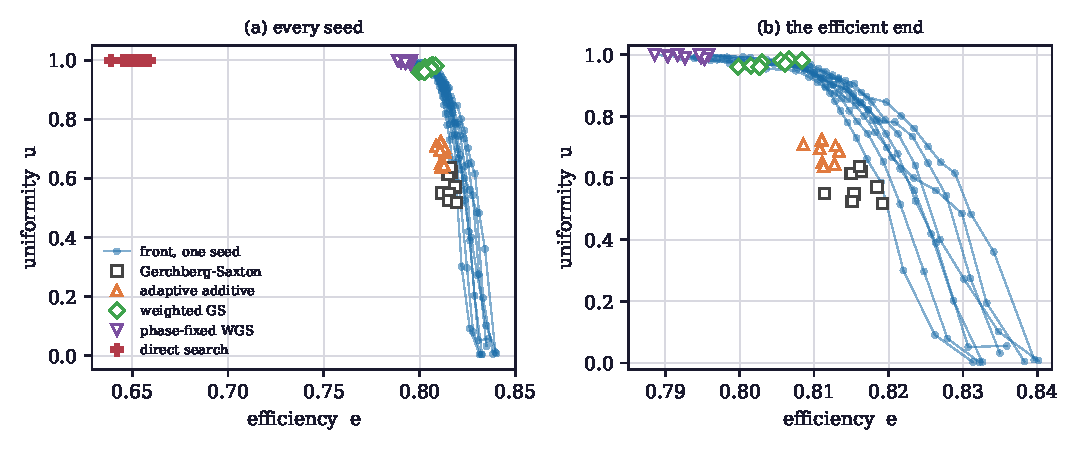
\includegraphics[width=\textwidth]{fig-front.pdf}
\caption{Fronts of the efficiency-uniformity trade-off on the ten by ten lattice for \nSeeds{} seeds (blue circles joined by lines) and the points of the five published methods on the same seeds (open and filled markers): (a) the whole plane, (b) enlarged near the efficient end. The front falls steeply from the uniform end, and the points of weighted GS, phase-fixed WGS and direct search sit near that end.}
\label{fig:front}
\end{figure}

\begin{table}[t]
\centering\small
\caption{Efficiency and uniformity (mean $\pm$ half-width of the 95 percent interval over \nSeeds{} seeds) of the points of the published methods and of the front on the ten by ten lattice, and the hypervolume with the reference $(0,0)$: for a single point it is $e\,u$, for the union of four points and for the front it is the area of Eq.~\ref{eq:hv}. The union is that of Gerchberg--Saxton, the adaptive additive iteration, weighted GS and direct search, without phase-fixed WGS.}
\label{tab:main}
\begin{tabular}{@{}lrrr@{}}
\toprule
Result & Efficiency & Uniformity & Hypervolume \\
\midrule
Gerchberg-Saxton & $0.816\pm0.002$ & $0.573\pm0.038$ & $0.468\pm0.031$ \\
Adaptive additive & $0.811\pm0.001$ & $0.682\pm0.027$ & $0.553\pm0.022$ \\
Weighted GS & $0.804\pm0.002$ & $0.972\pm0.008$ & $0.782\pm0.008$ \\
Phase-fixed WGS & $0.793\pm0.002$ & $0.995\pm0.004$ & $0.789\pm0.003$ \\
Direct search & $0.651\pm0.005$ & $0.999\pm0.000$ & $0.650\pm0.005$ \\
\midrule
Union of the four published points &  &  & $0.8071\pm0.0023$ \\
Front (knee point) & $0.793\pm0.002$ & $1.000\pm0.000$ &  \\
Front (whole) & 0.793 to 0.836 & 0.015 to 1 & $0.8223\pm0.0025$ \\
\bottomrule
\end{tabular}

\end{table}

The first hypothesis holds. The hypervolume of the front is \hvFront{} (interval \hvFrontCi) and that of the union of the four points is \hvPub{} (interval \hvPubCi), and the paired difference is \hvDiff{} with the interval \hvDiffLo{} to \hvDiffHi{}; it is positive in \hvGeCount{} of \nSeeds{} seeds, from \hvDiffMin{} in the weakest seed to \hvDiffMax{} in the strongest, which is a gain of \hvRatioPct{} percent of the union.
Adding phase-fixed WGS, the start of the front, to the union gives a hypervolume of \hvPubSeven{}, and the front still exceeds it by \hvDiffSeven{} (interval \hvDiffSevenLo{} to \hvDiffSevenHi) in \hvGeCountSeven{} of \nSeeds{} seeds. The union of the published points is not dominated by the front: the gain comes from the region of efficiency above the uniform end, where the front has points at intermediate uniformity that the published points leave empty, and not from a better uniform end. The second hypothesis holds: the front has \domGSMin{} to \domGSMax{} points that dominate the point of Gerchberg--Saxton (mean \domGSMean) and \domGAAMin{} to \domGAAMax{} that dominate the point of the adaptive additive iteration (mean \domGAAMean) in every seed, and
the number of seeds in which both are dominated is \domBothSeeds{} of \nSeeds{}. Direct search is dominated by one point of the front in \domDSSeeds{} of \nSeeds{} seeds, its efficiency of \ptDSE{} being the lowest of the five points.

The fourth hypothesis is not confirmed. The front has a dominating point for the point of weighted GS in only \domGSWSeeds{} of \nSeeds{} seeds (at most \domGSWMax{} points) and for the point of phase-fixed WGS in \domPFSeeds{} of \nSeeds{} (at most \domPFMax). The two points are the ones nearest the uniform end of the front: weighted GS has an efficiency of \ptGSWE{} and a uniformity of \ptGSWU{}, phase-fixed WGS \ptPFE{} and \ptPFU{}, while the front at the same efficiency has a lower uniformity. The reading is the risk that the research record named: the points of weighted GS are already near the best attainable corner on this task, and the front adds the efficient side of the trade-off and not a better uniform end.
The representative point of Eq.~\ref{eq:knee} is the uniform end in every seed, with an efficiency of \kneeE{} (interval \kneeELo{} to \kneeEHi) and a uniformity of \kneeU{}: because the efficiency rises by a few percent while the uniformity falls by a large factor, the product $eu$ is largest where the uniformity is one, so the knee rule returns the refined start and the information of the method is in the front and not in the knee.

\begin{figure}[t]
\centering
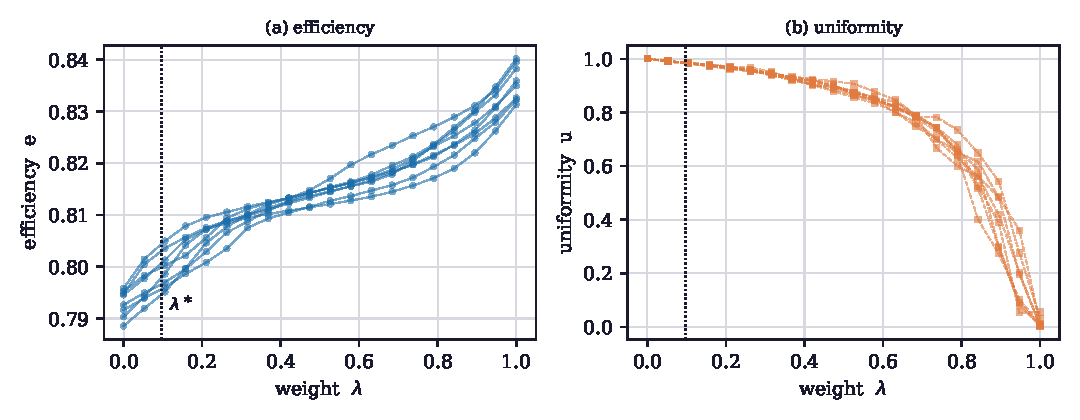
\includegraphics[width=\textwidth]{fig-lambda.pdf}
\caption{Efficiency (a) and uniformity (b) along the weight $\lambda$ for the \nSeeds{} seeds of the main experiment; the vertical dotted line is the mean value $\lambda^\ast$ of Eq.~\ref{eq:lamstar} computed from the largest efficiency of each front. The efficiency rises quickly up to about $\lambda=0.3$, slowly between 0.3 and 0.8 and quickly again near one; the uniformity falls slowly until $\lambda$ is near one, where it falls fast.}
\label{fig:lambda}
\end{figure}

Figure~\ref{fig:lambda} plots the two quantities against the weight. The efficiency increases monotonically with the weight in \monoESeeds{} of \nSeeds{} seeds, the error $E$ in \monoLossSeeds{} of \nSeeds{}, and the uniformity decreases monotonically in \monoUSeeds{} of \nSeeds{}, with at most \monoUViolMax{} step in which it rises in the remaining seed. This is the direction that Proposition~\ref{prop:mono}(a) predicts for global minimizers, here observed for the conjugate-gradient solutions. The weight at which the loss asks for the largest efficiency that is reached is
$\lambda^\ast=\lamSat{}$ (interval \lamSatLo{} to \lamSatHi). Beyond it the loss asks for more light than any hologram of the front delivers, and the front continues toward the efficient end: the efficiency still rises, up to a total gain of \eMaxFrontDelta{} over the start, and the uniformity falls from near one to near zero. The value of $\lambda^\ast$ is computed from the largest efficiency that each front reaches, so it restates that measurement as a weight and is not a prediction; the quantity that the proposition gives without a run is the upper bound $\lambda_1=\ablTargetLamMax{}$ (Section~\ref{sec:ablation}), which is well above the measured $\lambda^\ast$. The measured front shows that the supply keeps growing slowly after $\lambda^\ast$, at the price of the uniformity.

\subsection{Sensitivity to the reference point and one-parameter fronts of the published methods}\label{sec:res-rivals}

The hypervolume depends on the reference point. Table~\ref{tab:refs} repeats the comparison of the front and the published union with the reference $(0.5,0)$ and $(0.7,0)$, which discard the part of the plane below those efficiencies. The paired difference is \hvRefHalfDiff{} (interval \hvRefHalfLo{} to \hvRefHalfHi) and \hvRefSevenDiff{} (interval \hvRefSevenLo{} to \hvRefSevenHi) respectively, positive in \hvRefHalfGe{} and \hvRefSevenGe{} of \nSeeds{} seeds, so the ordering does not depend on the reference among the three tested. The size of the difference
is about the same in absolute terms for the three references, while the hypervolumes themselves shrink, so in relative terms the front's advantage grows as the reference moves toward the efficiencies at which the methods operate. The hypervolume with the reference $(0,0)$ is dominated by the high-uniformity region, where a point already covers most of the area, which is the weakness of the criterion that the acceptance test of the method inherits.

\begin{table}[t]
\centering\small
\caption{Hypervolume of the front and of the union of the four published points for three reference points, with the paired difference (mean $\pm$ half-width of the 95 percent interval over \nSeeds{} seeds). The ordering of the front and the union is the same for the three references.}
\label{tab:refs}
\begin{tabular}{@{}lrrr@{}}
\toprule
Reference of the hypervolume & Front & Published union & Difference, 95\% interval \\
\midrule
$(0,0)$ & $0.8223\pm0.0025$ & $0.8071\pm0.0023$ & $0.0152\pm0.0027$ \\
$(0.5,0)$ & $0.3223\pm0.0025$ & $0.3074\pm0.0023$ & $0.0149\pm0.0027$ \\
$(0.7,0)$ & $0.1223\pm0.0025$ & $0.1088\pm0.0020$ & $0.0135\pm0.0025$ \\
\bottomrule
\end{tabular}

\end{table}

A single point of a published method is a weak comparator, because each method has a knob that moves it. The one-parameter fronts of Section~\ref{sec:compared} give the published methods their best chance: the iterates of weighted GS and of phase-fixed WGS, and the sweep of the exponent of the adaptive additive iteration. Table~\ref{tab:rivals} gives their hypervolume. The front exceeds the weighted GS path by \rivGswDiff{} (interval \rivGswLo{} to \rivGswHi), the phase-fixed path by \rivPfDiff{} (\rivPfLo{} to \rivPfHi) and the adaptive additive sweep by \rivGaaDiff{} (\rivGaaLo{} to \rivGaaHi), in \rivGswGe{}, \rivPfGe{} and \rivGaaGe{} of \nSeeds{} seeds, and it exceeds the union of all of them and of the five points by \rivUnionDiff{} (interval \rivUnionLo{} to \rivUnionHi{}) in \rivUnionGe{} of \nSeeds{} seeds.
The fifth hypothesis therefore holds on the hypervolume. It does not mean that the front is better than the published methods point by point. Figure~\ref{fig:rivals} shows why. The iterates of weighted GS approach a point that lies on the uniform side of the front with a higher efficiency than the front has at the same uniformity: in seed 1, weighted GS after 100 iterations reaches an efficiency of \seedOneGswE{} at a uniformity of \seedOneGswU{}, while the front point of nearest efficiency (\seedOneNearE) has a uniformity of \seedOneNearU{}. Of the \nLambda{} points of the front, \frontDomMin{} to \frontDomMax{} (mean \frontDomMean) are dominated by at least one point of the published methods and their one-parameter fronts, and adding the published points to the front raises its hypervolume by only \hvGainPub{} on average (at most \hvGainPubMax). Of the 211 points of the three one-parameter fronts, \rivUndom{} on average per seed (at most \rivUndomMax) have no front point of equal or higher efficiency and uniformity, which says that the front does not cover the published iterates.

\begin{table}[t]
\centering\small
\caption{Hypervolume of the one-parameter fronts that the published methods give on the same seeds, the paired difference of the front from each (mean $\pm$ half-width of the 95 percent interval), and the number of seeds in which the front is at least as large. The last row is the union of the three fronts and of the five points.}
\label{tab:rivals}
\begin{tabular}{@{}lrrr@{}}
\toprule
One-parameter front of a published method & Hypervolume & Front minus it & Seeds front $\ge$ \\
\midrule
Weighted GS, iterates 1 to 100 & $0.8054\pm0.0020$ & $0.0169\pm0.0037$ & 8 of 8 \\
Phase-fixed WGS, iterates 1 to 100 & $0.7899\pm0.0034$ & $0.0324\pm0.0050$ & 8 of 8 \\
Adaptive additive, exponent 0 to 1 & $0.5880\pm0.0172$ & $0.2343\pm0.0158$ & 8 of 8 \\
Union of all of them and the five points & $0.8131\pm0.0012$ & $0.0092\pm0.0016$ & 8 of 8 \\
\bottomrule
\end{tabular}

\end{table}

\begin{figure}[t]
\centering
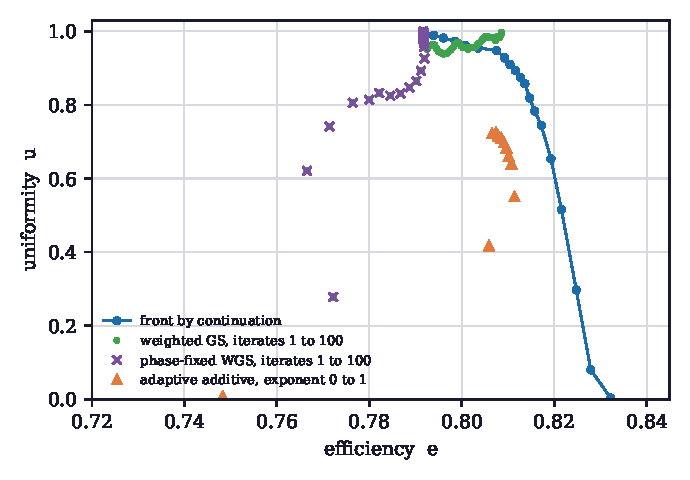
\includegraphics[width=0.78\textwidth]{fig-rivals.pdf}
\caption{The front of seed 1 (blue circles joined by a line) against the iterates 1 to 100 of weighted GS (green dots) and of phase-fixed WGS (purple crosses), and the adaptive additive iteration at 30 iterations with the exponent from 0 to 1 (orange triangles), on the ten by ten lattice. The last iterates of weighted GS lie above and to the right of the first points of the front.}
\label{fig:rivals}
\end{figure}

The dominance of part of the front by published iterates depends on the iteration budget and on the start, and not only on the loss: with 30 conjugate-gradient iterations per weight instead of 15 the mean number of dominated points falls from \ablDefaultDom{} to \ablCgThirtyDom{}, and when the front starts from the hologram of weighted GS after 100 iterations it falls to \ablStartGswHDom{} (Section~\ref{sec:ablation}), on the five seeds of the ablation. A direct comparison on the loss itself separates two explanations. The hologram of weighted GS after 100 iterations has a normalized error $E$ of \diagGswHundredE{} and a normalized light $S$ of \diagGswHundredS{} on the target of the seed, and for \diagGswHundredSeeds{} of \nSeeds{} seeds there is at least one weight at which its loss $L_\lambda$ is lower than that of the front
point (\diagGswHundredMin{} to \diagGswHundredMax{} weights, mean \diagGswHundredMean). The conjugate-gradient minimizer of the loss therefore stops, at those weights, in a point that is worse on the loss itself than a hologram that the fixed-point iteration of weighted GS reaches; the first part of the front inherits the basin of its start. The same comparison for phase-fixed WGS after 100 iterations gives \diagPfHundredSeeds{} of \nSeeds{} seeds with at least one weight (mean \diagPfHundredMean{} weights).

\subsection{What the weight does: the shifted target and the bounds}\label{sec:res-theory}

Figure~\ref{fig:shift}(a) draws the total light that the shifted target of Proposition~\ref{prop:shift} asks for, as a multiple of the efficiency of the start, and panel (b) plots the efficiency that the hologram reaches against it for the \nSeeds{} seeds. The two do not agree: the requested total grows with the weight without bound, while the efficiency reached stays within a few percent of the start. The measured efficiency at the largest weight is \eMaxFront{}, \eMaxRatio{} times the efficiency of the start, and the shifted target passes that value at the weight
$\lambda^\ast=\lamSat{}$. The gap between what is asked and what is delivered is the price of keeping the traps equal: the loss raises the target of every trap by the same amount, and a phase-only hologram on this task cannot follow it with a gain of more than \eMaxRatioPct{} percent in light.

\begin{figure}[t]
\centering
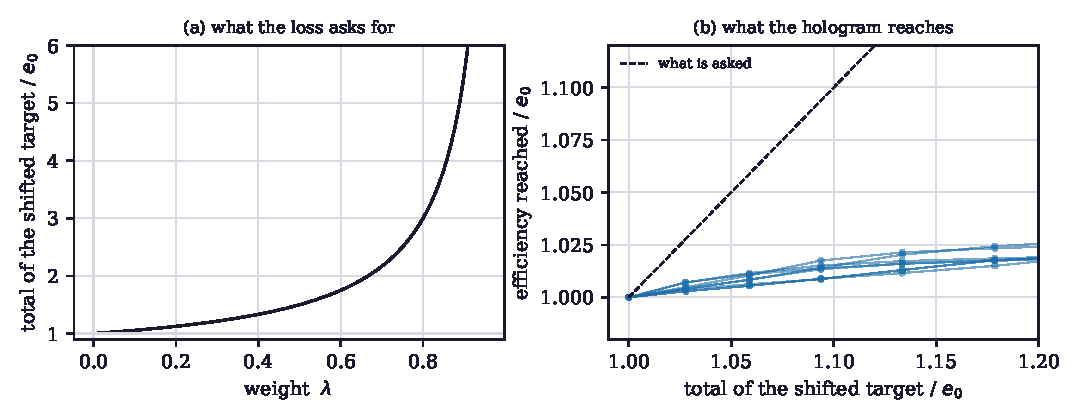
\includegraphics[width=\textwidth]{fig-shift.pdf}
\caption{(a) Total light of the shifted target of Proposition~\ref{prop:shift} as a multiple of the efficiency of the start, against the weight $\lambda$ (equal weights). (b) Efficiency reached by the hologram at each weight, as a multiple of the efficiency of the start, against the total that the target asks for, for the \nSeeds{} seeds; the dashed line is the case in which the hologram delivers what is asked.}
\label{fig:shift}
\end{figure}

The bounds of Proposition~\ref{prop:bound} hold on every front point of every seed. The smallest slack of the first bound, the bound minus the measured relative standard deviation in percent, is \sigmaSlackMin{}, which is positive and close to zero because the bound is an equality where the efficiency equals that of the start, as at the first point of each front. The smallest slack of the second bound is \uSlackMin{}; the bound is informative, that is, above zero, on \uBoundInf{} of the \uBoundPts{} front points of the main experiment, the ones with small error. Figure~\ref{fig:bound} plots the first bound.
A numerical check of the identity of Proposition~\ref{prop:shift} on random phases of a small array gives a largest absolute residual of \identResid{} over \identTrials{} trials and five weights, at the level of the rounding of the arithmetic.

\begin{figure}[t]
\centering
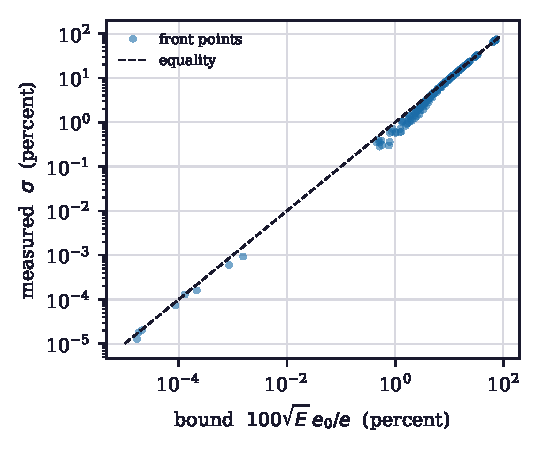
\includegraphics[width=0.62\textwidth]{fig-bound.pdf}
\caption{Relative standard deviation $\sigma$ of every front point of the main experiment (blue dots) against the bound of Proposition~\ref{prop:bound}, $100\sqrt E\,e_0/e$ (both in percent, logarithmic axes), and the line of equality (dashed). Every point is on or below the line; the points near the line are those whose efficiency is close to that of the start.}
\label{fig:bound}
\end{figure}

\subsection{Cost of the front}\label{sec:res-cost}

The third hypothesis concerns the time. Alone on the machine and with the module's own entry, the front takes \timeAloneMin{} to \timeAloneMax{} seconds for the three timed seeds (mean \timeAlone), so it is under the 60 seconds of the acceptance criterion in \timeAloneUnder{} of \timeAloneN{} seeds, with a margin that is thin on this machine and that the load of the machine changes. The record of the engine reports 16.6 seconds for the same task, a factor of about three below these times; this paper does not explain the factor: the timing here ran on a machine shared with other jobs (Section~\ref{sec:limits}), and the machine and the load of that record are not available to this paper, so the two times are not comparable and only the criterion of 60 seconds is read from the present ones. Over the \timeN{} runs of the ablation, the seconds in one thread are described by a line of $\timeSlope\,$ms
per conjugate-gradient iteration of one weight plus a constant of \timeIntercept{} seconds (coefficient of determination \timeRTwo), shown in Figure~\ref{fig:cost}. The constant is the part of the cost that does not scale with the weights and steps, mainly the start of 30 iterations of phase-fixed WGS, and the slope is the cost of one conjugate-gradient iteration, one to a few evaluations of the loss and its gradient; the linear model of Eq.~\ref{eq:cost} describes the measured time well. A direct search sweep on the same task takes \dsSec{} seconds in one thread, about as long as the whole front, and
the front returns \nParetoMean{} points where a sweep returns one.

\begin{figure}[t]
\centering
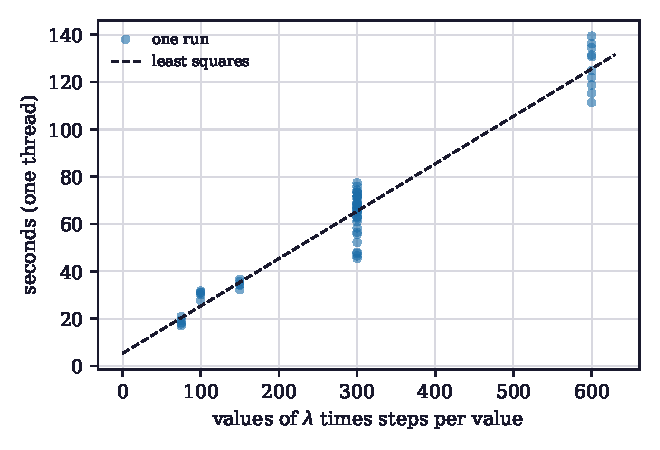
\includegraphics[width=0.62\textwidth]{fig-cost.pdf}
\caption{Seconds of one front in one thread against the number of weights times the conjugate-gradient iterations per weight, for the runs of the ablation (blue dots) and the least-squares line (dashed). The runs differ in the number of weights and the steps per weight; the line fits them with the coefficient of determination stated in the text.}
\label{fig:cost}
\end{figure}

\subsection{Other geometries: the benchmark and the bake}\label{sec:res-bench}

The benchmark of the studio stores a front for \benchNThirty{} of its geometries, obtained from the first seed with the converged budget, and the published points of the same geometry from the medians of the cells at 30 and 100 iterations on the ideal device. Table~\ref{tab:bench} gives the hypervolume of the stored front, that of the union of the four published points and the difference, and Figure~\ref{fig:bench} plots the difference. At 30 iterations the front meets the union on \benchPassThirty{} of \benchNThirty{}
geometries, with margins from \benchWorstThirty{} to \benchBestThirty{}. At 100 iterations it meets it on \benchPassHundred{} of \benchNHundred{}, with margins from \benchWorstHundred{} to \benchBestHundred{}, so the stored front lies below the union by at most \benchWorstAbsHundred{}. The eighth hypothesis is therefore refuted on the stored data at both budgets: the worst margin is \benchWorstThirty{} at 30 iterations and \benchWorstHundred{} at 100. Two facts qualify the result. The stored fronts are truncated: each ends at a weight below one (the largest stored weight is in Table~\ref{tab:bench}), which is consistent with the wall-clock limit of the converged
row of the benchmark, so the front misses the efficient tail that contributes to the hypervolume. And the medians of the published points are those of the cells of the benchmark, whose seeds depend on the wall-clock bound; the count of geometries at 100 iterations moved between runs of the benchmark of the same release, from 3 to 4 and to 0 in the record of the engine, and the file that is read here gives \benchPassHundred{}.

\begin{table}[t]
\centering\small
\caption{Hypervolume of the stored front of each benchmark geometry that has one, that of the union of the medians of the four published points (Gerchberg--Saxton, adaptive additive, weighted GS, direct search), and their difference, at 30 and at 100 iterations on the ideal device; the number of stored points and the largest stored weight are listed. Source: the committed benchmark file.}
\label{tab:bench}
\footnotesize\setlength{\tabcolsep}{3pt}
\begin{tabular}{@{}llrrrrr@{}}
\toprule
Geometry & Iter. & Points & Largest $\lambda$ & Front & Union & Difference \\
\midrule
G1 lattice 10 x 10 & 30 & 3 & 0.105 & 0.8352 & 0.8270 & +0.0082 \\
G2 ring, 36 traps & 30 & 7 & 0.368 & 0.7082 & 0.6966 & +0.0116 \\
G3 random, 100 traps & 30 & 6 & 0.263 & 0.7144 & 0.7041 & +0.0103 \\
G4 quasi-periodic, 119 & 30 & 5 & 0.211 & 0.7708 & 0.7643 & +0.0065 \\
G5 3D lattice 5 x 5 x 3 & 30 & 5 & 0.211 & 0.9012 & 0.8876 & +0.0136 \\
G6 large, 1024 and 819 & 30 & 1 & 0.000 & 0.7910 & 0.7916 & -0.0006 \\
G1 lattice 10 x 10 & 100 & 3 & 0.105 & 0.8352 & 0.8395 & -0.0043 \\
G2 ring, 36 traps & 100 & 7 & 0.368 & 0.7082 & 0.7017 & +0.0065 \\
G3 random, 100 traps & 100 & 6 & 0.263 & 0.7144 & 0.7106 & +0.0039 \\
G4 quasi-periodic, 119 & 100 & 5 & 0.211 & 0.7708 & 0.7718 & -0.0010 \\
G5 3D lattice 5 x 5 x 3 & 100 & 5 & 0.211 & 0.9012 & 0.8985 & +0.0026 \\
G6 large, 1024 and 819 & 100 & 1 & 0.000 & 0.7910 & 0.8037 & -0.0127 \\
\bottomrule
\end{tabular}

\end{table}

\begin{figure}[t]
\centering
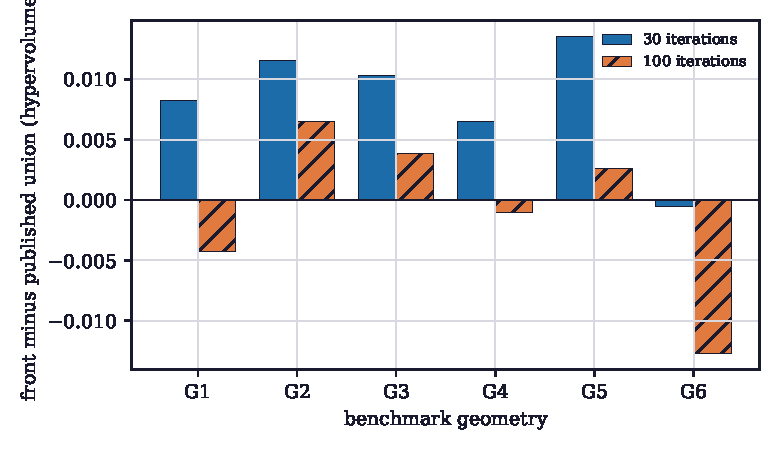
\includegraphics[width=0.8\textwidth]{fig-bench.pdf}
\caption{Hypervolume of the stored front minus that of the union of the four published points for each benchmark geometry, at 30 iterations (solid bars) and at 100 iterations (hatched bars). Bars above zero mean the front covers more area than the points; at 100 iterations \benchPassHundred{} of the \benchNHundred{} bars are at or above zero.}
\label{fig:bench}
\end{figure}

Table~\ref{tab:bake} lists the knee of the front that the studio's bake stores for the cases that run the method, as the mean and the interval over \bakeSeeds{} seeds. The knee is the refined start in the four cases (an efficiency near that of phase-fixed WGS on the cases of one plane and a uniformity near one), and the relative standard deviation is below one percent in every case listed, so the bake shows the uniform end of the front and not its trade-off.

\begin{table}[t]
\centering\small
\caption{Knee of the front stored by the studio's bake for the cases that run the method: efficiency, uniformity and relative standard deviation (mean $\pm$ half-width of the 95 percent interval over \bakeSeeds{} seeds; the intervals are wide with three seeds). Source: the committed file of measured ranges.}
\label{tab:bake}
\begin{tabular}{@{}lrrr@{}}
\toprule
Case & Efficiency & Uniformity & Relative std. dev. (percent) \\
\midrule
C01 & $0.801\pm0.066$ & $1.000\pm0.002$ & $0.03\pm0.13$ \\
C02 & $0.803\pm0.017$ & $0.989\pm0.030$ & $0.53\pm1.41$ \\
C05 & $0.895\pm0.015$ & $0.985\pm0.009$ & $0.66\pm0.39$ \\
C07 & $0.799\pm0.011$ & $0.990\pm0.017$ & $0.54\pm0.98$ \\
\bottomrule
\end{tabular}

\end{table}

\subsection{Outcome of each hypothesis}\label{sec:res-outcome}

The first, second, third, fifth, sixth and seventh hypotheses hold on the task of the acceptance test. The first holds with a paired difference of \hvDiff{} in \hvGeCount{} of \nSeeds{} seeds, the second in every seed, the third with a thin margin on the machine used, the fifth with the front above the union of the one-parameter fronts, the sixth with monotone efficiency and error in every seed and a uniformity that rises once in one seed, and the seventh with the cold start lower by the amount of Table~\ref{tab:ablation}.
The fourth is not confirmed: the weighted GS and phase-fixed points are dominated in \domGSWSeeds{} and \domPFSeeds{} of \nSeeds{} seeds. The eighth is refuted on the benchmark at both budgets. The scope of the result is therefore the following. On the ten by ten task the front adds the efficient side of the trade-off to the points of the published methods and exceeds the area that those points and their one-parameter fronts cover, and it does not improve on the weighted GS iterates at the uniform end, where
\frontDomMin{} to \frontDomMax{} of its points are dominated.

\section{Ablation}\label{sec:ablation}

The ablation varies one choice of the method at a time from the reference front (20 weights, 15 steps per weight, a linear schedule, a warm start along the weights, a start from phase-fixed WGS, the scaled loss) on the first \nSeedsAbl{} seeds, and reports the hypervolume of the variant, its paired difference from the reference, the lowest uniformity reached, and the seconds of one thread.
The reference has a hypervolume of \ablDefaultHv{} on these seeds and takes \ablDefaultSec{} seconds in one thread. Table~\ref{tab:ablation} gives the twelve variants and Figure~\ref{fig:ablation} plots the paired differences with their intervals. With five seeds the intervals are wide, and a difference whose interval contains zero is not distinguished from no change.

\subsection{Components of the method}\label{sec:abl-components}

\begin{table}[t]
\centering\small
\caption{Ablation of the front on the ten by ten task: hypervolume of each variant (mean $\pm$ half-width of the 95 percent interval over \nSeedsAbl{} seeds), its paired difference from the reference front, the lowest uniformity on the front and the seconds of one thread. The first row is the reference; every other row changes the one choice named in its first two columns.}
\label{tab:ablation}

\footnotesize\setlength{\tabcolsep}{3pt}
\begin{tabular}{@{}llrrrr@{}}
\toprule
Component & Variant & Hypervolume & Change & Lowest $u$ & Seconds \\
\midrule
Reference & 20 values, 15 steps, linear, warm & $0.8230\pm0.0036$ &  & 0.012 & 64.2 \\
Number of values & 5 values & $0.8130\pm0.0043$ & $-0.0100\pm0.0046$ & 0.015 & 18.7 \\
 & 10 values & $0.8188\pm0.0024$ & $-0.0042\pm0.0034$ & 0.029 & 34.7 \\
 & 40 values & $0.8242\pm0.0031$ & $0.0012\pm0.0017$ & 0.022 & 134.5 \\
Steps per value & 5 steps & $0.8190\pm0.0039$ & $-0.0040\pm0.0043$ & 0.058 & 30.3 \\
 & 30 steps & $0.8235\pm0.0030$ & $0.0005\pm0.0014$ & 0.013 & 118.5 \\
Schedule & quadratic in $\lambda$ & $0.8221\pm0.0036$ & $-0.0009\pm0.0003$ & 0.011 & 70.8 \\
 & target-spaced & $0.8133\pm0.0026$ & $-0.0097\pm0.0012$ & 0.944 & 70.6 \\
Continuation & cold start per value & $0.8134\pm0.0057$ & $-0.0096\pm0.0070$ & 0.020 & 72.7 \\
Start & plain GS start & $0.8170\pm0.0055$ & $-0.0060\pm0.0024$ & 0.019 & 68.2 \\
 & random, no iteration & $0.8143\pm0.0046$ & $-0.0087\pm0.0051$ & 0.012 & 59.8 \\
 & weighted GS, 100 it. & $0.8236\pm0.0028$ & $0.0006\pm0.0014$ & 0.017 & 48.0 \\
Loss scaling & unscaled loss & $0.8033\pm0.0065$ & $-0.0197\pm0.0081$ & 0.002 & 62.8 \\
\bottomrule
\end{tabular}

\end{table}

\begin{figure}[t]
\centering
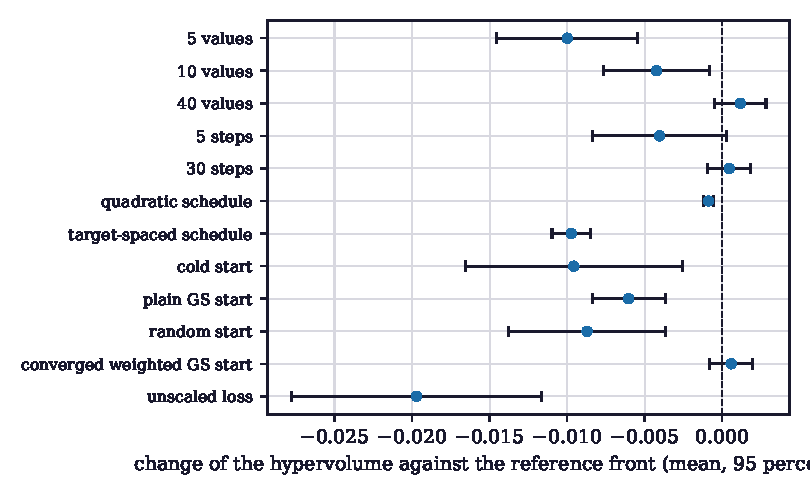
\includegraphics[width=0.84\textwidth]{fig-ablation.pdf}
\caption{Paired difference of the hypervolume of each variant from the reference front (points) with its 95 percent interval over \nSeedsAbl{} seeds (bars); variants are in the order of Table~\ref{tab:ablation}. Intervals that do not reach the dashed zero line are differences that five seeds distinguish from no change.}
\label{fig:ablation}
\end{figure}

\paragraph{The continuation.} A cold start, in which every weight begins from the refined start and not from its neighbour, lowers the hypervolume by \ablColdDiff{} (interval \ablColdDiffLo{} to \ablColdDiffHi), at the same cost. The efficiency that the cold front reaches at the largest weight is \ablColdEMax{} against \ablDefaultEMax{} for the warm front,
because fifteen steps from the start cannot travel as far as fifteen steps from a neighbour that has already travelled; and the number of its points that published iterates dominate rises from \ablDefaultDom{} to \ablColdDom{}. This is the measured form of Proposition~\ref{prop:warm}: the warm start spends its steps on a correction of the order of the step in the weight. The seventh hypothesis holds.
The same reading explains the two variants that vary the work per weight. With 5 steps per weight the hypervolume changes by \ablCgFiveDiff{} (interval \ablCgFiveDiffLo{} to \ablCgFiveDiffHi) and with 30 steps by \ablCgThirtyDiff{} (\ablCgThirtyDiffLo{} to \ablCgThirtyDiffHi); both intervals contain zero, so the default of 15 is on a plateau of the hypervolume, and the 30 steps cost \ablCgThirtySec{} seconds against \ablDefaultSec{}, nearly twice as much, for a change that five seeds do not distinguish from none.
The number of weights matters more at the low end: 5 weights lower the hypervolume by \ablNLamFiveDiff{} (\ablNLamFiveDiffLo{} to \ablNLamFiveDiffHi) and 10 weights by \ablNLamTenDiff{} (\ablNLamTenDiffLo{} to \ablNLamTenDiffHi), because the front is then a polygon with few vertices and the area under it is underestimated, while 40 weights change it by \ablNLamFortyDiff{} (\ablNLamFortyDiffLo{} to \ablNLamFortyDiffHi), again within the interval of no change, at \ablNLamFortySec{} seconds.
So the hypervolume is already resolved at 20 weights, and the number of points on the front is the only thing that more weights buy.

\paragraph{The start.} The front depends on the hologram from which it starts, because that hologram sets the total light $e_0$ of the target. Starting from 30 iterations of plain GS lowers the hypervolume by \ablStartGsDiff{} (\ablStartGsDiffLo{} to \ablStartGsDiffHi), starting from the random superposition with no iteration by \ablStartRandDiff{} (\ablStartRandDiffLo{} to \ablStartRandDiffHi), and both are distinguished from no change.
Starting from the hologram of weighted GS after 100 iterations, which has a higher efficiency than the phase-fixed start (the first point of the front has a mean efficiency of \ablStartGswHEFirst{} against \ablDefaultEFirst{}), changes the hypervolume by \ablStartGswHDiff{} (\ablStartGswHDiffLo{} to \ablStartGswHDiffHi), which is no change at this number of seeds, and removes the domination of the front by published iterates: the number of dominated points falls from \ablDefaultDom{} to \ablStartGswHDom{}. The choice of the start of the module is therefore sound for the hypervolume and is
not the best choice for the uniform end, where a better-converged start gives a better first part of the front at no cost in area.

\subsection{Schedule of the weights and scaling of the loss}\label{sec:abl-schedule}

\begin{figure}[t]
\centering
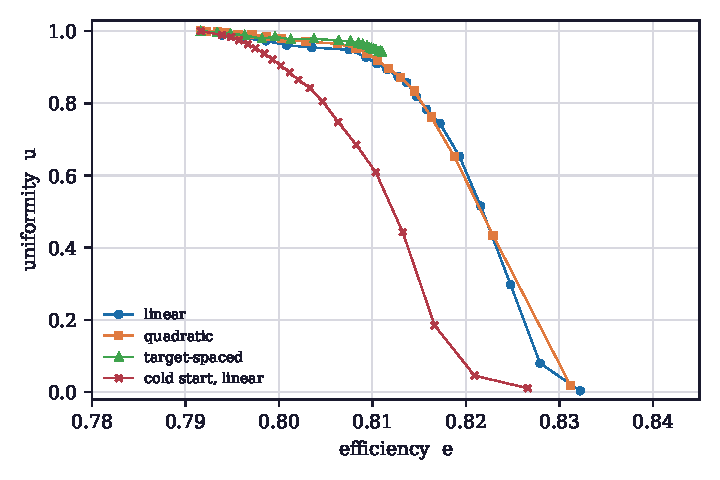
\includegraphics[width=0.78\textwidth]{fig-schedule.pdf}
\caption{Front of seed 1 for the linear schedule of the weights (blue circles), the quadratic schedule (orange squares), the target-spaced schedule of Proposition~\ref{prop:shift} (green triangles) and the cold start with the linear schedule (red crosses), on the ten by ten lattice. The target-spaced schedule covers the uniform end more finely and stops near the efficiency of 0.81; the cold start trails the others in efficiency at equal uniformity.}
\label{fig:schedule}
\end{figure}

The quadratic schedule, dense near the uniform end, changes the hypervolume by \ablQuadDiff{} (interval \ablQuadDiffLo{} to \ablQuadDiffHi); the interval excludes zero, and the size is a tenth of a percent, so the schedule is a second-order choice. The target-spaced schedule, the one that Proposition~\ref{prop:shift} suggests, lowers the hypervolume by \ablTargetDiff{} (\ablTargetDiffLo{} to \ablTargetDiffHi), and Figure~\ref{fig:schedule} shows why: it spaces its 20 points evenly in the total light that the target asks for,
from the efficiency of the start up to a total of one, which corresponds to weights up to \ablTargetLamMax{}; the front it returns stops at a largest efficiency of \ablTargetEMax{} and a lowest uniformity of \ablTargetUMin{}, and it omits the efficient tail that the linear schedule reaches (\ablDefaultEMax{} and \ablDefaultUMin{}). The schedule resolves the useful part of the front well, with uniformity above 0.94, and it is the better choice
when the useful part is the question; it gives a lower hypervolume because the criterion counts the tail, so the schedule is a matter of the purpose of the front. The prediction of the proposition that most points of a linear grid fall beyond $\lambda^\ast$ is correct, and the cost of it is small in area terms.

The scaling of the loss is the largest effect in the table. Without the two divisions the shift $\delta_\lambda$ of Proposition~\ref{prop:shift} is $\lambda/(2(1-\lambda))$ per trap, which is \rawFactor{} times (the factor $M/e_0$) the shift of the scaled loss at the same weight, so at the first weight after the origin, $\lambda=\ablRawLamOne{}$, the loss asks for a raise of every trap by \rawShiftRel{} times its intensity, and the front collapses: the mean uniformity at that weight is \ablRawFirstU{} and every later point has a uniformity of at most \ablRawLaterU{}; the hypervolume is lower by \ablRawDiff{} (\ablRawDiffLo{} to \ablRawDiffHi) and only \ablRawNPar{} of the points are non-dominated on average. The efficiency
at the efficient end is the same, \ablRawEMax{} against \ablDefaultEMax{}, so what the scaling buys is the middle of the front. The normalization is the reason that one weight means the same on every array, and this variant measures what its absence costs on the task.

\subsection{What each component contributes}\label{sec:abl-summary}

In the order of the size of the effect, the unscaled loss costs \ablRawDiff{}, the target-spaced schedule \ablTargetDiff{}, the cold start \ablColdDiff{}, the random start \ablStartRandDiff{}, the plain GS start \ablStartGsDiff{} and 5 weights \ablNLamFiveDiff{}, all lower than the reference and all excluded from zero by their intervals. The components that carry the front are therefore the normalization of the loss, the warm start along the weights and a start that is already close to uniform. The number of steps per weight and the number of weights above 20 are
on a plateau, and the converged start of weighted GS does not change the area. The surprising outcome is the start: the module's start is not the best start for the part of the front near the uniform end, which a front computed from weighted GS after 100 iterations covers without domination, and the area is the same.
Two further readings follow from the table. The seconds of the variants follow the number of weights and of steps, as the cost model of Section~\ref{sec:complexity} says, and the start from weighted GS after 100 iterations is the cheapest of the full-length variants, \ablStartGswHSec{} seconds against \ablDefaultSec{}.
And the lowest uniformity of the variants that reach $\lambda=1$ lies between \ablRawUMin{} (unscaled loss) and \ablCgFiveUMin{} (5 steps per weight), against \ablTargetUMin{} for the target-spaced schedule that stops earlier, so the tail of the front is set by the weight and its depth by the steps.

\section{Discussion}\label{sec:discussion}

\subsection{Why the results are what they are}\label{sec:disc-why}

The shape of the front is set by one fact that Proposition~\ref{prop:shift} and Figure~\ref{fig:shift} expose: the loss can ask for as much light as it likes, and the hologram can deliver only \eMaxRatioPct{} percent more than the start (\eMaxRatio{} times the efficiency of the start at the largest weight). Every extra percent of efficiency is paid for by a large drop of uniformity, so the front is steep and the useful part of the trade-off, where the uniformity is still at least 0.9, spans an increase of the efficiency of
only \eGainUNinePp{} percentage points. This is why the single points of weighted GS and phase-fixed WGS, which sit at the uniform end, are already close to the best that the task allows, and why the hypervolume with the reference $(0,0)$ is dominated by that end: a point $(e,u)$ near $(0.8,1)$ covers $0.8$ of an area whose total is one. The hypervolume of the front exceeds that of the union of the published points by \hvDiff{} not because the uniform end improved but because the front adds points of
higher efficiency at intermediate uniformity, where no published point lies. The sensitivity analysis with the references $(0.5,0)$ and $(0.7,0)$ shows that the advantage is robust (\hvRefHalfRel{} and \hvRefSevenRel{} percent of the union against \hvRatioPct{} percent), and that it is larger in relative terms the more the reference discounts the uniform end. A reader who cares about the uniform end only should read the dominance counts and not the hypervolume.

The front also depends on its start. The ablation shows that the start from phase-fixed WGS is better than a start from plain GS or from the random superposition, and the diagnostic shows that it is not the best possible: weighted GS after 100 iterations reaches a hologram with more light in the traps at nearly the same flatness, and the loss itself is lower for that hologram than for the front at \diagGswHundredMin{} to \diagGswHundredMax{} of the weights. The conjugate-gradient iteration with 15 steps per weight does not leave the basin of its start, and the first part of the front
is that of the basin of phase-fixed WGS, whose efficiency is lower than that of the converged iterates of weighted GS. When the front starts from the converged hologram no front point is dominated and the hypervolume is unchanged within the interval. The loss is not convex, the stationarity of Proposition~\ref{prop:mono}(b) is a necessary condition only, and the engine's front is a set of local solutions: the warm start keeps them on one branch, which the monotone counts of Section~\ref{sec:res-front} support, and does not make the branch the best one.

The ablation reads consistently with the theory. The cold start loses because the warm start's initial gradient is proportional to the step in the weight (Proposition~\ref{prop:warm}); the unscaled loss loses because it asks for a raise of the traps that is $M/e_0=\rawFactor{}$ times larger at the same weight, which Proposition~\ref{prop:shift} makes explicit through the constant $\delta_\lambda$, proportional to $\sum T^2/e_0$; and the plateau in the steps per weight and the number of weights above 20 follows from a front that is smooth.

\subsection{Failure cases and negative results}\label{sec:disc-failures}

Four results of the paper are negative or partial and are reported as such. First, the front does not dominate the point of weighted GS or of phase-fixed WGS in most seeds: the fourth hypothesis is not confirmed, and on this task the continuation adds the efficient side of the trade-off and not a better uniform end. Second, \frontDomMin{} to \frontDomMax{} of the \nLambda{} points of the front are dominated by iterates that the published methods reach, in particular by weighted GS after 100 iterations,
so the set that the front draws is an inner approximation of the attainable set, not the Pareto front of the problem; the converged start removes the domination with no change in area that five seeds can resolve, and the module as it stands does not use it. Third, the stored fronts of the benchmark meet the published union on \benchPassHundred{} of the \benchNHundred{} geometries at 100 iterations (the margins run from \benchWorstHundred{} to \benchBestHundred{}) and on \benchPassThirty{} of \benchNThirty{} at 30 iterations; the stored fronts end at weights well below one (the largest stored weight of each geometry is in Table~\ref{tab:bench}), which is consistent with the 20 seconds that the benchmark's converged row allows for 300 iterations per weight, they hold between one and seven points, and the published medians at 100 iterations are those of the cells, so the comparison favours the published points. The count at 100 iterations moved between runs of the benchmark of the same release, from 3 to 4 to 0 in the record of the engine, which is the reading that this paper offers for a margin that is at most \benchWorstAbsHundred{} in absolute value in the file read here. Fourth, the knee rule of Eq.~\ref{eq:knee} returns the uniform end in \kneeZeroSeeds{} of \nSeeds{} seeds, so the single hologram that the engine returns is the
refined start and the front is the product of the method; and the target-spaced schedule, which the theory suggests, loses \ablTargetDiff{} of hypervolume because it stops short of the efficient tail.

Two results are positive but narrower than they look. The hypervolume gain of \hvDiff{} is the same in the three reference points tested in absolute terms and is positive in every seed, but it is computed against four points of the published methods and their one-parameter fronts, not against the best attainable set, which the front does not reach. And the time of the front, \timeAloneMin{} to \timeAloneMax{} seconds alone on this machine, is under the 60 seconds of the acceptance criterion with a thin margin, while a direct search sweep takes \dsSec{} seconds and returns one point.

\subsection{What the results imply for use}\label{sec:disc-use}

For an experimenter who needs a hologram of a trap array, the method gives a picture that the single-point methods do not: the cost in light of each step of uniformity, and the position of the published points relative to it. On the ten by ten task the picture says that weighted GS or phase-fixed WGS is the right choice if uniformity matters at all, because the extra \eMaxRatioPct{} percent of light costs almost all of the uniformity, and that GS and the adaptive additive iteration are inside the front. The front is worth computing when a decision depends on how much uniformity can be given up for light: when the power budget is tight, when the traps are shallow and the atoms
are loaded only if the depth is sufficient, or when an array larger than the task changes the position of the weighted GS point; the paper does not measure those cases, and the benchmark shows that on all six of its geometries, the ten by ten lattice included, the stored front is not above the published union at 100 iterations.

For the studio and for the method, the results suggest four changes that the paper does not implement. The start of the front should be the converged hologram of weighted GS and not 30 iterations of phase-fixed WGS, which removes the dominated points. The knee rule should not be the product $eu$ but a point that the user selects, or the largest efficiency subject to a uniformity floor. The converged row of the benchmark should give the front the weights it needs, since a stored front that ends at a weight of 0.05 cannot be compared with a union of points. And a device model should be put in the loss, as the crosstalk
and quantization models of the literature~\cite{schroff,persson} allow, because every number of this paper is for the ideal device.

\section{Limitations}\label{sec:limits}

\subsection{Threats to validity}\label{sec:threats}

\paragraph{Internal validity.} The intervals come from \nSeeds{} seeds for the main experiment, \nSeedsAbl{} for the ablation and three for the timing, and a Student interval with so few seeds is wide; a difference whose interval contains zero is not distinguished from none, which is the case for the steps per weight, the weights above 20 and the converged start. The seeds fix the random superposition that starts every method, so the pairing by seed removes the variation of the start,
and what it leaves is the variation of the optimization. The conjugate-gradient iteration is stopped after 15 steps per weight and the loss is not convex, so the solutions are local and the monotonicity of Proposition~\ref{prop:mono}(a), proved for global minimizers, is observed and not guaranteed. The diagnostic of Section~\ref{sec:res-rivals} shows the consequence: the solutions at \diagGswHundredMin{} to \diagGswHundredMax{} of the weights are worse on the loss than a hologram of weighted GS.
The loop of the ablation is a copy of the module's loop; it is checked against the module on the first seed (largest absolute difference \consistMax{}) and for the other seeds it is the same code path, so a difference between the two on another seed is possible but was not looked for. The seconds of the main experiment come from processes with one thread, and the seconds of the timing from a machine shared with other jobs.
The dominance criterion of Eq.~\ref{eq:ndom} is the one of the module's test, with a strict inequality in the uniformity only, so a front point that ties a published point in the efficiency and exceeds it in the uniformity counts, and one that ties in the uniformity does not.

\paragraph{External validity.} The experiment is one task: a ten by ten lattice of equal traps in one plane, on a 256 pixel SLM padded by 2, with one wavelength and one lens, on the ideal device. The benchmark extends the check to five other geometries, but only through the stored fronts and the cell medians, which were not produced for this comparison: the stored front is the front of the first seed with a converged budget that the wall-clock bound shortens, and the published points are medians over a number of seeds that
the same bound sets. The result on the benchmark is mixed: at 100 iterations the stored front meets the union of the published points on \benchPassHundred{} of \benchNHundred{} geometries, so the claim of the paper does not extend beyond the acceptance task. The bake lists four cases with three seeds each. No hardware was used: the uniformities of the paper are those of the scalar model and not of an instrument, and the published points are computed by the engine's implementation of each method, not by the code of its authors.
Arrays with unequal weights, traps in several planes, vortex traps and the device with crosstalk, quantization and flicker are outside what was measured for the method; the weights $w_m$ enter the loss and the metrics, but the bounds of Proposition~\ref{prop:bound} are proved only for equal weights.

\paragraph{Construct validity.} The method optimizes the normalized squared error $E$ and the normalized light $S$, and the paper evaluates the front in the plane of the efficiency $e$ and the uniformity $u$. The uniformity depends on the brightest and dimmest traps only and the error on all traps, so the two are related by the inequalities of Proposition~\ref{prop:bound} and not by a function, and a front of $(E,-S)$ is not guaranteed to be a front in $(e,u)$; the readout keeps the non-dominated points of the second plane, and
the number that remains is \nParetoMean{} of \nLambda{} on average. The hypervolume with the reference $(0,0)$ is dominated by the uniform end; three references were tested and the ordering did not change, but a reference chosen by an experimenter for a particular array can weigh the parts of the front differently. The efficiency is the light in the traps as a fraction of the input power, which is the quantity of the foundational comparison and not the diffraction efficiency of an instrument.

\subsection{Scope and what is not claimed}\label{sec:scope}

The paper claims the following and no more. On the ten by ten task of the engine, on the ideal device, a continuation of the normalized weighted loss from the output of phase-fixed WGS, with 20 weights and 15 conjugate-gradient steps per weight, gives a front whose hypervolume exceeds that of the union of the points of four published methods in every one of \nSeeds{} seeds, and that dominates two of those points in every seed. It does not claim that the front is the Pareto front of the problem: part of it is
dominated by iterates of weighted GS. It does not claim an improvement at the uniform end, over the weighted GS point or over the phase-fixed point, where it dominates them in a minority of seeds. It does not claim an improvement on the geometries of the benchmark, where the stored front meets the published union on \benchPassHundred{} of \benchNHundred{} geometries at 100 iterations. It does not claim a time advantage: the time is of the order of one minute on the machine used and depends on its load. It does not claim a result for a device model, for unequal weights, for traps off the
focal plane or for hardware. The identity of Proposition~\ref{prop:shift} and the bounds of Proposition~\ref{prop:bound} are proved and checked numerically, and they hold for every hologram; the monotonicity of Proposition~\ref{prop:mono}(a) is proved for global minimizers and observed for the local ones; Conjecture~\ref{conj:branch} is supported by the counts of Section~\ref{sec:res-front} and by the cold start of the ablation, and is not proved.

\section{Reproducibility}\label{sec:repro}

The method, the engine, the benchmark and the scripts of this paper are in the repository named in the header block, at the release that carries the engine module \texttt{b5\_pareto} and the benchmark of \benchRows{} rows. Every number of the text is a macro of the file \texttt{data/b5\_numbers.tex}, every table is a file written by the same script, and every figure is a vector file written by a second script from the same data file. Nothing in the text is typed from a run.
The numbers are rebuilt from the repository root with the pipeline environment of the engine by
\begin{verbatim}
.venv-pipeline/Scripts/python.exe \
  manuscripts/efficiency-uniformity-front/data/measure.py \
  --seeds 8 --seeds-abl 5 --seeds-timing 3
.venv-notebooks/Scripts/python.exe \
  manuscripts/efficiency-uniformity-front/figures/make_figs.py
pdflatex -output-directory <build folder> \
  manuscripts/efficiency-uniformity-front/tex/main.tex
\end{verbatim}
where the third command is run three times for the references. The measurement script runs the parts \texttt{main}, \texttt{rivals}, \texttt{ablation}, \texttt{identity}, \texttt{stored}, \texttt{diagnostic} and \texttt{timing} and writes \texttt{data/b5.json}; the option \texttt{--macros-only} rewrites the macro and table files from that file without running the engine, and \texttt{--only-variants} adds ablation variants to it.
The first part checks that its own copy of the loop reproduces the module's front for the first seed; the largest absolute difference between the two fronts is \consistMax{}. The seeds are the integers $1,\dots,\nSeeds$ for the main experiment, $1,\dots,\nSeedsAbl$ for the ablation and $1,2,3$ for the timing, and each seed fixes the random superposition that starts every method.

The run times are those of one machine with 32 logical processors that was shared with other jobs while the measurement ran. The parallel parts ran in processes of one thread each, and the time of a front in those processes is the \timePool{} seconds of the main experiment. The timing part runs the module's own entry alone, in one process with the threads of the machine, for three seeds, and the front takes \timeAloneMin{} to \timeAloneMax{} seconds, mean \timeAlone{}. The research record of the engine reports 16.6 seconds for the same task
on a machine under contention, so the figure depends on the load of the machine more than on the method. The benchmark and the bake are read as committed: the file of the benchmark carries its own protocol, with 300 iterations or 20 seconds for its converged row and up to 600 seconds of wall clock per group of seeds, so its cell medians depend on the seeds that the bound admits, and a re-run of the benchmark can change the margins of Table~\ref{tab:bench}. The data of the main experiment, the front and the points of every seed are in \texttt{data/b5.json}, which is the archive of the measurement.

\section{Conclusions}\label{sec:conclusions}

A continuation over the weight of a normalized loss computes, for one array of point traps, a front of efficiency against uniformity of about \nLambda{} points in under a minute, with a closed-form gradient and a warm start along the weights. On a ten by ten lattice of 100 traps its hypervolume is \hvFront{} against \hvPub{} for the union of the points of Gerchberg--Saxton, the adaptive additive iteration, weighted GS and direct search, a paired difference of \hvDiff{} (95 percent interval \hvDiffLo{} to \hvDiffHi) over \nSeeds{} seeds, and it exceeds the union of the one-parameter fronts of the published methods by \rivUnionDiff{}.
The front dominates the points of Gerchberg--Saxton and of the adaptive additive iteration in every seed, and it adds to the published points the efficient side of the trade-off: the efficiency rises by at most \eMaxRatioPct{} percent over the start while the uniformity falls from one to near zero, so the cost of light in uniformity is steep. Proposition~\ref{prop:shift} gives the weight its reading, the squared error against a uniformly raised target, and the weight $\lambda^\ast=\lamSat{}$ beyond which the target exceeds the efficiency that is reached;
Proposition~\ref{prop:bound} ties the spread and the uniformity to the loss and holds on every front point.

The result is partial. The weighted GS point and the phase-fixed point are dominated by the front in \domGSWSeeds{} and \domPFSeeds{} of \nSeeds{} seeds, \frontDomMin{} to \frontDomMax{} of the points of the front are dominated by iterates of weighted GS, and the stored fronts of the benchmark of the studio are below the published union at 100 iterations on all \benchNHundred{} geometries, with a deficit of at most \benchWorstAbsHundred{}. The ablation shows that the warm start, the scaling of the loss and a start close to uniform carry the front (each raises the hypervolume by between \ablStartGsAbs{} and \ablRawAbs{} against its removal), that the steps per weight and the weights above 20 are on a plateau, and that a start from the converged hologram of weighted GS removes the domination without changing the area.

The next steps follow from these limits: start the front from the converged hologram of weighted GS; replace the knee rule by a choice of the user; give the stored fronts the weights that they need in the benchmark; put the device model of the literature in the loss, so that the front is computed for the device that displays the hologram and not for the ideal one; and measure the front on an instrument, where the trade-off between the light in the traps and their uniformity decides how many atoms an array can load.


\begin{thebibliography}{99}\small
\bibitem{dileonardo} R. Di Leonardo, F. Ianni and G. Ruocco, ``Computer generation of optimal holograms for optical trap arrays,'' \emph{Optics Express} 15(4), 1913, 2007. \url{https://doi.org/10.1364/OE.15.001913}.
\bibitem{polin} M.~Polin, K.~Ladavac, S.-H.~Lee, Y.~Roichman and D.~G.~Grier, ``Optimized holographic optical traps,'' \emph{Opt. Express} 13(15), 5831, 2005. \url{https://doi.org/10.1364/OPEX.13.005831}.
\bibitem{kim2019} D.~Kim \emph{et al.}, ``Large-scale uniform optical focus array generation with a phase spatial light modulator,'' \emph{Opt. Lett.} 44(12), 3178, 2019. \url{https://doi.org/10.1364/OL.44.003178}.
\bibitem{kimoe2019} H.~Kim, M.~Kim, W.~Lee and J.~Ahn, ``Gerchberg--Saxton algorithm for fast and efficient atom rearrangement in optical tweezer traps,'' \emph{Opt. Express} 27(3), 2184, 2019. \url{https://doi.org/10.1364/OE.27.002184}.
\bibitem{pasienski} M. Pasienski and B. DeMarco, ``A high-accuracy algorithm for designing arbitrary holographic atom traps,'' \emph{Optics Express} 16(3), 2176, 2008. \url{https://doi.org/10.1364/OE.16.002176}.
\bibitem{harte} T. Harte, G. D. Bruce, J. Keeling and D. Cassettari, ``Conjugate gradient minimisation approach to generating holographic traps for ultracold atoms,'' \emph{Optics Express} 22(22), 26548, 2014. \url{https://doi.org/10.1364/OE.22.026548}.
\bibitem{bowman} D.~Bowman \emph{et al.}, ``High-fidelity phase and amplitude control of phase-only computer generated holograms using conjugate gradient minimisation,'' \emph{Opt. Express} 25(10), 11692, 2017. \url{https://doi.org/10.1364/OE.25.011692}.
\bibitem{schroff} P. Schroff, A. La Rooij, E. Haller and S. Kuhr, ``Accurate holographic light potentials using pixel crosstalk modelling,'' \emph{Scientific Reports} 13, 3252, 2023. \url{https://doi.org/10.1038/s41598-023-30296-6}.
\bibitem{persson} M. Persson, D. Engstr\"om and M. Goks\"or, ``Reducing the effect of pixel crosstalk in phase only spatial light modulators,'' \emph{Optics Express} 20(20), 22334, 2012. \url{https://doi.org/10.1364/OE.20.022334}.
\bibitem{nogrette} F.~Nogrette \emph{et al.}, ``Single-atom trapping in holographic 2D arrays of microtraps with arbitrary geometries,'' \emph{Phys. Rev. X} 4(2), 021034, 2014. \url{https://doi.org/10.1103/PhysRevX.4.021034}.
\bibitem{whyte} G. Whyte and J. Courtial, ``Experimental demonstration of holographic three-dimensional light shaping using a Gerchberg--Saxton algorithm,'' \emph{New Journal of Physics} 7, 117, 2005. \url{https://doi.org/10.1088/1367-2630/7/1/117}.
\bibitem{chakravarthula} P.~Chakravarthula, Y.~Peng, J.~Kollin, H.~Fuchs and F.~Heide, ``Wirtinger holography for near-eye displays,'' \emph{ACM Trans. Graph.} 38(6), 1--13, 2019. \url{https://doi.org/10.1145/3355089.3356539}.
\bibitem{peng} Y.~Peng, S.~Choi, N.~Padmanaban and G.~Wetzstein, ``Neural holography with camera-in-the-loop training,'' \emph{ACM Trans. Graph.} 39(6), 1--14, 2020. \url{https://doi.org/10.1145/3414685.3417802}.
\bibitem{eybposh} M. H. Eybposh, N. W. Caira, M. Atisa, P. Chakravarthula and N. C. P\'egard, ``DeepCGH: 3D computer-generated holography using deep learning,'' \emph{Optics Express} 28(18), 26636, 2020. \url{https://doi.org/10.1364/OE.399624}.
\bibitem{shi} L. Shi, B. Li, C. Kim, P. Kellnhofer and W. Matusik, ``Towards real-time photorealistic 3D holography with deep neural networks,'' \emph{Nature} 591, 234--239, 2021. \url{https://doi.org/10.1038/s41586-020-03152-0}.
\bibitem{manetsch} H.~J.~Manetsch, G.~Nomura, E.~Bataille, X.~Lv, K.~H.~Leung and M.~Endres, ``A tweezer array with 6,100 highly coherent atomic qubits,'' \emph{Nature} 647, 60--67, 2025. \url{https://doi.org/10.1038/s41586-025-09641-4}.
\bibitem{ebadi} S.~Ebadi \emph{et al.}, ``Quantum phases of matter on a 256-atom programmable quantum simulator,'' \emph{Nature} 595, 227--232, 2021. \url{https://doi.org/10.1038/s41586-021-03582-4}.
\bibitem{chew} Y.~T.~Chew \emph{et al.}, ``Ultraprecise holographic optical tweezer array,'' \emph{Phys. Rev. A} 110(5), 053518, 2024. \url{https://doi.org/10.1103/PhysRevA.110.053518}.
\bibitem{das1998} I. Das and J. E. Dennis, ``Normal-boundary intersection: a new method for generating the Pareto surface in nonlinear multicriteria optimization problems,'' \emph{SIAM Journal on Optimization} 8(3), 631--657, 1998. \url{https://doi.org/10.1137/S1052623496307510}.
\bibitem{das1997} I. Das and J. E. Dennis, ``A closer look at drawbacks of minimizing weighted sums of objectives for Pareto set generation in multicriteria optimization problems,'' \emph{Structural Optimization} 14(1), 63--69, 1997. \url{https://doi.org/10.1007/BF01197559}.
\bibitem{zitzler1999} E. Zitzler and L. Thiele, ``Multiobjective evolutionary algorithms: a comparative case study and the strength Pareto approach,'' \emph{IEEE Transactions on Evolutionary Computation} 3(4), 257--271, 1999. \url{https://doi.org/10.1109/4235.797969}.
\bibitem{zitzler2003} E. Zitzler, L. Thiele, M. Laumanns, C. M. Fonseca and V. G. da Fonseca, ``Performance assessment of multiobjective optimizers: an analysis and review,'' \emph{IEEE Transactions on Evolutionary Computation} 7(2), 117--132, 2003. \url{https://doi.org/10.1109/TEVC.2003.810758}.
\bibitem{deb} K. Deb, A. Pratap, S. Agarwal and T. Meyarivan, ``A fast and elitist multiobjective genetic algorithm: NSGA-II,'' \emph{IEEE Transactions on Evolutionary Computation} 6(2), 182--197, 2002. \url{https://doi.org/10.1109/4235.996017}.
\bibitem{beume} N. Beume, C. M. Fonseca, M. Lopez-Ibanez, L. Paquete and J. Vahrenhold, ``On the complexity of computing the hypervolume indicator,'' \emph{IEEE Transactions on Evolutionary Computation} 13(5), 1075--1082, 2009. \url{https://doi.org/10.1109/TEVC.2009.2015575}.
\bibitem{allgower} E. L. Allgower and K. Georg, \emph{Numerical Continuation Methods}, Springer Series in Computational Mathematics, Springer, 1990. \url{https://doi.org/10.1007/978-3-642-61257-2}.
\bibitem{miettinen} K. Miettinen, \emph{Nonlinear Multiobjective Optimization}, International Series in Operations Research and Management Science, Springer, 1998. \url{https://doi.org/10.1007/978-1-4615-5563-6}.
\bibitem{nocedal} J. Nocedal and S. J. Wright, \emph{Numerical Optimization}, Springer Series in Operations Research and Financial Engineering, Springer, 2006. \url{https://doi.org/10.1007/978-0-387-40065-5}.
\bibitem{hillermeier} C. Hillermeier, ``Generalized homotopy approach to multiobjective optimization,'' \emph{Journal of Optimization Theory and Applications} 110(3), 557--583, 2001. \url{https://doi.org/10.1023/A:1017536311488}.
\bibitem{fliege} J. Fliege and B. F. Svaiter, ``Steepest descent methods for multicriteria optimization,'' \emph{Mathematical Methods of Operations Research} 51(3), 479--494, 2000. \url{https://doi.org/10.1007/s001860000043}.
\bibitem{desideri} J.-A. D\'esid\'eri, ``Multiple-gradient descent algorithm (MGDA) for multiobjective optimization,'' \emph{Comptes Rendus Math\'ematique} 350(5--6), 313--318, 2012. \url{https://doi.org/10.1016/j.crma.2012.03.014}.
\bibitem{sener} O.~Sener and V.~Koltun, ``Multi-task learning as multi-objective optimization,'' Neural Information Processing Systems (NeurIPS), 2018; arXiv:1810.04650. \url{https://arxiv.org/abs/1810.04650}.
\bibitem{lin} X.~Lin, H.-L.~Zhen, Z.~Li, Q.~Zhang and S.~Kwong, ``Pareto multi-task learning,'' 33rd Conference on Neural Information Processing Systems (NeurIPS), 2019; arXiv:1912.12854. \url{https://arxiv.org/abs/1912.12854}.
\bibitem{navon} A.~Navon, A.~Shamsian, G.~Chechik and E.~Fetaya, ``Learning the Pareto front with hypernetworks,'' International Conference on Learning Representations (ICLR), 2021; arXiv:2010.04104. \url{https://arxiv.org/abs/2010.04104}.
\end{thebibliography}


\end{document}
